\begin{savequote}[85mm]
    Nothing travels faster than the speed of light, 
    with the possible exception of bad news, which obeys its own special laws.
    \qauthor{Douglas Adams}
    \end{savequote}


\chapter{Research Methods to Improve Data Quality}\label{chap:goal1}
This chapter focuses on enhancing data quality through innovative research methods. Firstly, the utilization of synthetic data generation, as detailed in sections \ref{subsec:gans}, \ref{subsec:tabular}, and \ref{subsec:similarity}, serves a dual purpose: expanding the volume of available data while simultaneously safeguarding privacy. This approach focuses on  techniques such as \acp{gan} to create realistic, yet non-sensitive data sets. Secondly, the development of automatic data quality assessment methods, explored in section \ref{subsec:dq}, marks a significant stride in ensuring the integrity and reliability of data. These methods aim to automate the process of evaluating data quality, thus reducing manual effort and increasing the efficiency and accuracy of data analysis.



\section{Can GANs Help Create Realistic Datasets?}\label{subsec:gans}
This section is based on the paper entitled "GANs for Tabular Healthcare Data Generation: A Review on Utility and Privacy". It focuses on a review of the \ac{gan} framework for creating synthetic data for healthcare. Tries to compile the metrics used for comparing and assessing synthetic data in terms of utility - or how similar they are to the original data and privacy - how protective of the patient's data it is. 

% !TeX root = ../thesis.tex

\subsection{Introduction}

With the growing technological advances, the quantity of healthcare-related data produced around the world increased exponentially \cite{choi_generating_2017,henry_adoption_2016}.
Consequently, the potential for harvesting this data also increases. The value locked within
this data could help provide better healthcare with new information about diseases,
drugs, and preventive therapies. It can also help create better \acp{his}, meaning an overall better clinical practice \cite{ISI:000502534100049}. But for this to happen, data must reach capable hands at the right time.
But the release of clinical data has several barriers attached and rightly so. The leakage of patient’s privacy can break the confidence of the population in healthcare
professionals and institutions. Patient safety
and privacy should be kept at all costs. However, the current mechanisms for privacy maintenance are very long, bureaucratic, and time-consuming, nationally \cite{comissao_nacional_protecao_de_dados_principios_2015}, and internationally \cite{office_for_civil_rights_guidance_2013}. The current scenario and general methods for privacy safeguards are related to pseudo-anonymisation techniques.
The removal of certain attributes, identifier modification, code grouping, or discretization are some methodologies. But not even these are totally safe \cite{el_emam_systematic_2011}.
Synthetic data appear as an alternative for clinical data sharing, promising great data
utility with minimal privacy concerns. Synthetic data is data that is generated automatically through programmatic processes. This is especially impactful for the case at hand
since synthetic data has no explicit connection with the original data. There are several
mechanisms for data synthesis postulated by \cite{goncalves_generation_2020}, there are
process-driven methods and data-driven methods. Process-driven methods generate
data through pre-determined models inputted into the generator. Data-driven methods
produce new data based on inputted source data. With this, it is possible to create new
patient data that has no relation to reality while providing the same statistical relations
between variables. This provides the basis for quality clinical research on top of this
new data. Even though these techniques are still new and in rapid development, the
results seem interesting \cite{goncalves_generation_2020}, but not without questions and doubts
\cite{stadler_synthetic_2020}.
Creating a thorough survey based on the generation of synthetic data is seldom a simple task when compared to other surveys since synthetic data is present across several domains and has several uses, like software testing, assessing methods, or generating hypotheses. Moreover, synthesis has
the double meaning of summing up information and generating something, easily wielding hundreds of results per query. Finally, trying to filter
algorithms aimed at tabular data is also burdensome, since not always it is easy to discriminate input types. These factors make the survey interesting to focus on the state-of-the-art mechanisms of generating tabular data.

\subsection{Theoretical background}
First introduced in 2014, \acp{gan} \cite{goodfellow_generative_2014} have been under the scope and have been proven very good for generating complex data. Images, text, and video have been successfully generated with very good performances. %cite?
The original architecture is based on two artificial neural networks trained simultaneously in a competitive manner. One of them, the generator, has the objective of generating the most realistic possible data, while the second network – the discriminator, has the opposite aim of aiming to distinguish the realistic data from the synthetic
data the best it can. So, the elegance of this architecture is that each network tries to
make the other perform better every time. The \ac{gan} architecture is shown in \ref{fig:gan-arch}.
% w - \omega
% θ - \theta
% G - generator
% D - discriminator

\begin{figure}
\centering
%\includegraphics[width=\textwidth]{image.png}
\includegraphics[scale=0.75]{figures/image.png}

\caption{\ac{gan} framework} \label{fig:gan-arch}
\end{figure}
The generator is represented by $G_{\theta}$ where the parameter $\theta$ represents the weights of
the neural network. It takes as input, a Gaussian random variable, and outputs $G_{\theta}$(Z).
Distribution of $G_{\theta}$(Z) is denoted by $P_{\theta}$. The goal of the generator is to choose $\theta$ such that the output $G_{\theta}$(Z) has a distribution close to the real data. The discriminator is represented by $D_{\omega}$, parametrized by weights $\omega$. The goal of the discriminator is to assign 1 to the samples from the real distribution $P_{X}$ and 0 to the generated samples ($P_{\theta}$). So, \acp{gan} can be mathematically represented by a \textit{MinMax} game identified by:
\begin{equation}
\min_{G}\max_{D} \; E [log(D_{\omega}(X)) + log(1-D_{\omega}(G_{\theta}(Z))]
\end{equation}
So, $G$ must minimize this equation and $D$ must maximize it, each one tweaking the weights of its network ($\theta$ and $\omega$) to do so. This is the loss function on the initial \ac{gan} architecture. After the classification of $D$, the $G$ is trained again with the error signal from $D$ through backpropagation. This equation is the log of the probability of $D$ predicting that the real data is genuine and the log probability of $D$ classifying synthetic data as not genuine. The equation is essentially the same as minimising the \ac{jsd} \cite{goodfellow_generative_2014}:
\begin{equation}
\min_{G} JS(P_{x}||P_{\theta})
\end{equation}
Where the JS means the \acl{jsd} between the probability of the real data and the probability of the generated data. The JS divergence provides a measure of the distance between two probability distributions. Therefore, the minimization over $\theta$ means, choosing the $P_{\theta}$ that is closest to the target distribution $P_{X}$ in the JS divergence distance. Despite the significant results provided by \acp{gan} with continuous real values, categorical values still seem to be a problem for this approach \cite{kusner_gans_2016}, since it is not directly applicable for calculating the gradients of latent categorical variables in order to train these networks through backpropagation. This happens since the output of the generator, even though can be transformed into a multinomial distribution with a \textit{softmax} layer, sampling from it is not a differentiable operation, limiting the backpropagation process of the \ac{gan}.

%One of the most famous alternative GAN architectures is the \textit{Wasserstein}  GAN (WGAN)
%\cite{arjovsky_wasserstein_2017} . It improves GAN by using the \textit{Wasserstein} distance instead of the \textit{Jensen-shannon divergence}. It is represented by the
%following minimax game:
%\begin{equation}
%\min_{G}\max_{\omega \; \epsilon \;W} \;\; E[f_{\omega}(X)] - E[f_{\omega}(G_{\theta}(Z))] 
%\end{equation} 
%Where functions $f_{\omega} \;  \omega \; \epsilon \;W$  are all \textit{K-Lipschitz} (with respect to $x$) for some K.
%This was proposed because it helps prevent mode collapse, where the generator maps
%several inputs to the same output. An example of this is a generator that starts creating
%several images with the same patterns or colours. The fact that this loss function can be
%very customisable in distinct GAN implementation, applying different functions can
%lead to different outcomes and architectures.

%\iffalse
%\subsubsubsection{Differential privacy}
%The privacy model most used in generative models is differential privacy \cite{dwork_differential_2006}. It is a mathematical model for measuring privacy loss. The basis of it is a mechanism that adds noise to a dataset through randomisation. Applying differential privacy is a method for guaranteeing that adding or removing any record from the original data does not influence the generation output. The formal definition, as stated in \cite{dwork_differential_2006} is:
%\begin{equation}
%Pr[M(x)\; \epsilon \; S] \leq e^\varepsilon Pr[M(y)\; \epsilon \; S] + \delta
%\end{equation} 
%Where M is a randomised mechanism, $\varepsilon$ is the privacy budget (balance between privacy and utility). The $x$ and $y$ represent adjacent datasets that differ on only one record. So, we say that M gives $\varepsilon$-differential privacy if the probability of seeing an event S in the $x$ dataset is at most equal to $e^\varepsilon$ multiplied by the probability that we see S when the dataset is $y$. Variable $\delta$ is the probability of an uncontrolled breach. With this, a smaller $\varepsilon$ will yield better privacy but a less accurate response, so it can be used to tweak the utility and privacy of the dataset.
%\fi

\subsection{Methods}
This search was made between December 2020 and January 2021. It was made on “Web of Science”, IEEE, PubMed, Arxiv and finally GitHub. The terms searched were related to \acp{gan}, synthetic data generation, electronic health records, patient data, or tabular data. Applications of \acp{gan} to non-tabular data were filtered, like image, sound, video, or graphs. Time series and text data were also removed since the methodology for synthesizing this type of data has specific functions related to the nature of the data. The filter for date was after 2014 since \acp{gan} were introduced at that time. The queries used were similar to the one below, adapted for the search mechanics for each website.


\begin{scriptsize}

{\fontfamily{courier}\selectfont
("generation" OR "creation" OR "synthesis" OR "synthesizing" OR "generating" OR "creating") AND ("synthetic data" OR "synthetic patient" OR "synthetic electronic health record" OR "synthetic EHR" OR "realistic patient data" OR "realistic health record" OR ("synthetic" AND "privacy" AND "utility"))  AND ("GAN" OR "Generative Adversarial Network")}
\end{scriptsize}
%\begin{verbnobox}[\scriptsize]
%("generation" OR "creation" OR "synthesis" OR "synthesizing" OR
%"generating" OR "creating") AND ("synthetic data" OR
%"synthetic patient" OR "synthetic electronic health record" 
%OR "synthetic EHR" OR "realistic patient data" OR "realistic 
%health record" OR ("synthetic" AND "privacy"  AND "utility")) 
%AND ("GAN" OR "Generative Adversarial Network")
%\end{verbnobox}

From the total articles found (1165) with all the queries, 100 articles were chosen for full text and in the end, 22 papers with \ac{gan} implementations that were tested on tabular data were selected. 
%These implementations were studied and evaluated in terms of privacy concerns and utility performance and compared when possible. 
%For selecting the articles and helping with paper selection, RAYYAN QCRI online \cite{rayyan:14:cochrane} was used along with Mendeley Reference Manager for paper management.


\subsection{Results}
The selected papers ranged from 2017 to 2020. Being that 2 are from 2017, 4 from 2018, 8 from 2019 and 8 from 2020. All authors showed original \ac{gan} implementations, apart from 2 papers. Beaulieu-Jones et al. \cite{beaulieu-jones_privacy-preserving_2019} used a
\ac{gan} architecture that was originally published with usage on image datasets \cite{odena_conditional_2017}. Additionally, Vega-Marquez et al.  \cite{ISI:000490706700022} used an already known implementation of conditional \acp{gan} \cite{mirza_conditional_2014}. We classified papers regarding 3 metrics: utility, privacy and clinical. For utility, we looked for  methods for measuring the generated data's quality. As for privacy, we aimed for some mechanism for measuring the privacy loss of the new data. Concerning clinical metrics, any kind of evaluation from healthcare professionals was considered. This can be seen in table \ref{tab:review_gans}.


\begin{table}[tphb]
\caption{Summary of the articles selected. The year, acronym, reference and  type of metrics mentioned are indicated. Code repository is mentioned when such information was provided. }\label{tab:review_gans}
\centering
\small
\begin{tabular}{lllclc}
%\begin{tabular}{l|llclc}

\toprule
 ID & year  & Acronym & Article & Metric & Code \\

% & \multicolumn{1}{|c}{Year \hspace{2 mm}}  & \multicolumn{1}{|c|}{Acronym} & \multicolumn{1}{c}{\hspace{2 mm} Article \hspace{1 mm}} & \multicolumn{1}{|c|}{Metric} & \multicolumn{1}{c|}{\hspace{2 mm}Code \hspace{2 mm}}  \\

\midrule
1 & 2017 & medGAN  &\cite{choi_generating_2017}          & Utility, Privacy, Clinical \hspace{1 mm} &  \cite{medGANurl}  \\

2 & 2017 & POSTER & \cite{ISI:000440307700174} & Utility, Privacy  &   \cite{POSTERurl}\\

3 & 2018 & table-GAN & \cite{park_data_2018} & Utility, Privacy         &   \cite{table-GAN-url} \\

4 & 2018 & dp-GAN & \cite{xie_differentially_2018}& Utility, Privacy &   \cite{dp-GAN-url}  \\

5 & 2018 & mc-medGAN & \begin{tabular}[c]{@{}l@{}}\cite{camino_generating_2018}\end{tabular}    & Utility &   \cite{mcmedgan-url}\\

6 & 2018 & TGAN &  \cite{xu_synthesizing_2018}& Utility &  \cite{tgan-url}\\

7 & 2019 & PATE-GAN & \begin{tabular}[c]{@{}l@{}}\cite{jordon_pate-gan_2019}\end{tabular}    & Utility, Privacy   & --\\

8 & 2019 & SPRINT-GAN & \cite{beaulieu-jones_privacy-preserving_2019}           & Utility, Privacy, Clinical &  \cite{sprint-GAN-url} \\

9 & 2019 & GAN-based &     \cite{ISI:000524576200016} & Utility, Privacy & --\\

10 & 2019 & CTGAN &  \cite{xu_modeling_2019} & Utility & \cite{CTGAN-url}\\

11 & 2019 & WGAN-DP & \begin{tabular}[c]{@{}l@{}}\cite{brenninkmeijer_generation_2019}\end{tabular} & Utility, Privacy    & \cite{WGAN-DP-url} \\

12 & 2019 & PPGAN &  \cite{liu_ppgan_2019} & Utility, Privacy &  \cite{ppgan-url}\\

13 & 2019 & medBGAN &   \cite{ISI:000502534100049} & Utility & --\\

14 & 2019 & medWGAN& \cite{medwgan}& Utility &  \cite{medWGAN-url}  \\

15 & 2020 & ADS-GAN& \begin{tabular}[c]{@{}l@{}}\cite{ISI:000557358500024}\end{tabular} & Utility, Privacy& --\\

16 & 2020 & corGAN & \cite{2001.09346}& Utility, Privacy &  \cite{corGAN-url}\\
17 & 2020 & CGAN &  \cite{ISI:000490706700022}& Utility& --\\

18 & 2020 & DPAutoGAN&  \cite{tantipongpipat2020differentially}& Utility, Privacy & \cite{DPAutoGAN-url}\\

19 & 2020 & GAN Boosting& \cite{2007.11934} & Utility, Privacy &  \cite{postganurl}\\

20 & 2020 & RDP-CGAN&  \cite{rdp-gan}& Utility, Privacy &  \cite{rdp-cgan-url}\\

21 & 2020 & WCGAN-GP&  \cite{WCGAN-GP}& Utility, Privacy & --\\
22 & 2020 & SMOOTH-GAN &  \cite{smooth-gan} & Utility & \cite{smooth-gan-url}\\
\bottomrule
\end{tabular}
\end{table}


The metrics the authors used are exhibited in table \ref{tab:results_review}. Regarding privacy, 15 papers assessed it or included some kind of mechanism to improve data protection. The most common was including Differential Privacy (DP) in the generation process. Other mechanisms for measuring privacy loss were Membership Inference (Member. Inf.), Attributes Disclosure (Attrib. Disc.), Euclidean distance (Eucl.), record-linkage (R. Linkage) and \acf{knn}.
As for utility, all papers assessed it. There were 3 major areas of utility assessment: Dimension-wise (DW) probability, cross-testing, and distance metrics. The most basic one was dimension-wise probability, which is important for making sanity checks for the generated data, comparing the distributions of each column between real and synthetic. In this category, we can find \textit{Bernoulli} (Bern.), cumulative distributions (Cumul. Dist.), \textit{Pearson} correlation (Pearson) and \textit{Spearman} correlation (Spearman), correlation coefficients (CCS), chi-squared test ($\chi^{2}$),  \acf{ks} or Correlation Matrices (Corre. Mat.).
Cross-testing was about training machine-learning algorithms with both datasets in order to compare the results. The key factor is generating a synthetic dataset based on the training set and then training models on the original training set and the generated dataset. Then the models are compared regarding their predictive capability on the (real) test set. This was a way of assessing if the generator models were capturing inter-variable relationships. The authors applied different metrics from \acf{auroc}, F1, \ac{auprc}, Accuracy (Acc.) to \acf{mre}. Finally, there was also the application of distance metrics, for measuring the difference between column distribution in both datasets. \acf{jsd}, \textit{Wasserstein} Distance (WD), \textit{Bhattacharyya} Distance (BD) or Generate Scores (GS) that was a metric implemented by the authors of \cite{liu_ppgan_2019} that creates a metric based on the sum of the mean of \textit{kullblack-leibler}  distance of all columns. Other less used methods were \acf{pca}, propensity score mean squared error ratio (pMSE). Normalised Mutual Information (NMI), which is the ability to capture correlations between columns by computing the pairwise mutual information and MMD (Maximum Mean Discrepancy), which is similar to distance metrics were also used. Regarding datasets utilized, the most used was MIMIC-III \cite{mimiciii} (9 times). The papers used 27 different datasets, being 16 healthcare-related and 11 non-healthcare related. 
Finally, regarding clinical evaluation, only two papers assessed it, as it is possible to see in table \ref{tab:review_gans}. Both had a group of clinicians assessing a sample of both real and synthetic information and evaluating from 0 to 10, where 10 is the most realistic.
One major point preventing a larger comparison is that despite some papers using the same dataset and same methodologies, the presented values are different, making it difficult for a clear comparison of results. One example is a dimension-wise prediction with F1 score for MIMIC-III. CorGAN presents the mean difference between the two classifications (real on real and synthetic on synthetic), while medBGAN presents the correlation coefficients of the two, and medGAN only presents the visual comparisons. Regarding code availability, 16 papers had the code publicly available in some form. As of January 2021, papers pointed in table \ref{tab:review_gans} have public code.



\begin{landscape}
\renewcommand{\arraystretch}{1.02} %add more space between cells (1.2 is a factor)
\begin{table}[htbp]
\caption{Summary of different metrics utilised for evaluating synthetic data. Grouped by utility and privacy metrics. Acronyms indicate the source paper} \label{tab:results_review} 

\begin{tabular}{p{26mm} p{84mm} p{60mm}}
\hline
Acronym & Utility & Privacy \\
\hline
medGAN	& \begin{enumerate*}
    \item Bern.
    \item Pred F1
\end{enumerate*} & \begin{enumerate*}
\item Attrib. disc. \item Memb. inf. \item KNN	\end{enumerate*}  \\

%\arrayrulecolor{mygrey}\hline

POSTER &	\begin{enumerate*}
\item Pred Acc.
\item Corre. Mat. \item BD
\end{enumerate*} & DP\\
table-GAN &	\begin{enumerate*}
\item Cumul. Dist.
\item Pred F1$\vert$MRE
 \end{enumerate*} &	\begin{enumerate*} \item Eucl.
\item Member. inf.   \end{enumerate*}  \\

dp-GAN &	\begin{enumerate*} \item Pred AUC \item Bern. \end{enumerate*} &	DP	 \\

mc-medGAN & 	\begin{enumerate*} \item Pred F1$\vert$AUC \item Bern. \item ME F1$\vert$Acc\end{enumerate*} & -- 	\\

TGAN &	\begin{enumerate*} \item KNN \item NMI \item Pred F1 \end{enumerate*} & --\\

PATE-GAN & \begin{enumerate*} \item  Pred AUC$\vert$AUPRC \end{enumerate*}	& DP \\
SPRINT-GAN & \begin{enumerate*}	\item Pred AUC \item Corre. Mat. \end{enumerate*} &	DP \\

GAN-based &	  \begin{enumerate*} \item Pred Acc. \item Corre. Mat. \end{enumerate*} & \begin{enumerate*} \item Hit. Rate \item R. Linkage  \item Eucl. \end{enumerate*} \\

CTGAN &	\begin{enumerate*} \item Pred F1$\vert$R2$\vert$Acc. \end{enumerate*} &  --\\

WGAN-DP &	\begin{enumerate*} \item Corre. Mat.
 \item PCA \item  Pearson RMSE\newline\item Pred F1$\vert$RMSE$\vert$1-MAPE(F1)  \end{enumerate*}  & \begin{enumerate*} \item Eucl. \item Dupl. \item DP \end{enumerate*}	\\

PPGAN &	\begin{enumerate*} \item GS \end{enumerate*}	& DP \\

medBGAN	& \begin{enumerate*}  \item Assoc. Rul.
 \item  CCS Pred F1
\item KS
 \end{enumerate*}	& -- \\

medWGAN	& \begin{enumerate*} \item Assoc. Rul.\item  CCS Pred F1 \item KS \end{enumerate*} & -- \\

ADS-GAN &  \begin{enumerate*} \item $\chi^{2}$ \item JSD \item WD
\item t-test \item Pred AUROC\newline
\item Corre. Mat. \end{enumerate*}	& DP \\

CorGAN &	\begin{enumerate*} \item Pred F1 \item Bern. \end{enumerate*}
 &	Member. Inf. \\

CGAN &	\begin{enumerate*} \item Pearson
\item Spearman \item Pred F1$\vert$AUC$\vert$Acc \end{enumerate*}  &	-- \\

DPAutoGAN & \begin{enumerate*} \item Pred AUROC$\vert$$R^2$  \item Bern. \end{enumerate*}	
 &	DP \\
GAN Boosting & \begin{enumerate*} \item pRMSE \item Pred AUROC$\vert$AUPRC$\vert$Acc. \end{enumerate*}	
	& DP \\
RDP-CGAN & \begin{enumerate*} \item Pred F1$\vert$AUROC$\vert$AUPRC \item MMD  \end{enumerate*}	
	& DP \\
WCGAN-GP & \begin{enumerate*} \item Corre. Mat.
 \item Pred F1  \end{enumerate*} & \begin{enumerate*} \item Dupl.
\item Eucl. \end{enumerate*} \\
SMOOTH-GAN & \begin{enumerate*} \item DW MAE \item Pearson  \item Pred AUROC$\vert$AUPRC \end{enumerate*}	
	& -- \\
\hline

\end{tabular}
\end{table}
\end{landscape}



%\begin{figure}[h]
%\centering
%\includegraphics[scale=0.50]{Paper_plot.png}
%\includegraphics[scale=0.54]{Rplot01.jpeg}

%\caption{Datasets used for measuring Utility and Privacy.} \label{fig2}
%\end{figure}



\subsection{Implications for future research}
From the work done in this paper, it is clear that synthetic data generation is a growing field. The increasing number of papers through the years as the growing quality in the mechanisms of generating data and assessing its quality is clear proof. 
It also became apparent that privacy and utility in synthetic data represent a delicate balance. The very same definition of differential privacy represents it. The compromise between privacy and utility is real and should be taken into account when creating privacy-demanding datasets.
Creating statistically good tabular datasets is already possible, but that task becomes increasingly difficult if privacy concerns are added. 
However, privacy is also a complex subject, and the context of the setting is important for privacy assessment, which explains the different approaches for evaluating privacy protection of synthetic data.
From this review, we believe that a proper evaluation of synthetic data generators in the healthcare setting with privacy concerns should at least include utility and privacy evaluations. For utility, we believe that evaluating column-wise is a nice first check but insufficient alone.
For table-wise, since there is no fundamental metric for assessing the inter-column correlations between mixed-type variables, cross-testing is the best next thing. Distance metrics are nice to have and seem to have the potential for creating a table-wise metric \cite{metrics}, so presenting them is important. Second, for privacy evaluation, we believe that Differential Privacy in itself is not a guarantee of protection for real patients. More research and depth should be employed when presenting results for such generators; record-linkage and attribute disclosure can provide extra guarantees.
Thirdly, a clinical evaluation should be done as well to understand if the synthetic patients are a reality in the clinical setting. Since the correlations could be correct but clinically (or biologically) they might not make sense. Finally, in the scope of this paper, only \acp{gan} were assessed, but there are more mechanisms for generating data, and could be interesting to assess how all of them perform on the same datasets. There are other methods for handling the mixed data types that regularly appear in clinical settings, like \acp{vae} Gaussian Mixtures, \ac{bn}, and imputation mechanisms, making them excellent candidates for this assessment.



\subsection{Conclusion}
In this paper, we had the opportunity to survey the current framework for generating tabular data using \acp{gan} and which ones were already tested in the healthcare setting. We summarised the utility and privacy metrics employed, and the datasets used to measure them. We analysed the code availability and made suggestions for further work on cataloguing, comparing, and assessing synthetic health data generators. A survey with a global benchmark of methodologies, despite being arduous, could yield great results for the community and take the aim of this paper further.

\section{How Can We Compare Two Tabular Datasets?}\label{subsec:tabular}
This section is based on the paper entitled "Dataset Comparison Tool: Utility and Privacy". This work followed the work on section \ref{subsec:gans}, where we compiled ways of assessing the utility of synthetic data. We understood that the mechanisms were far from consensual and a tool could be of use to merge all of this into a single file and report about data. Our purpose was to facilitate health data owners and legal responsible to understand how similar and protective a dataset was regarding the original one.

% !TeX root = ../thesis.tex

\subsection{Introduction}
Synthetic data can be defined as data that has no connection with a real-world phenomenon or event. It did not originate from a process in the real world, but rather a synthetic one. The idea is that synthetic data can have similar properties with real data, without needing to have an independent process for its generation.
Synthetic data has been used over the years for several usages, but in healthcare is still not very used. However, this scenario seems to be changing. It can be used for several use cases namely \cite{synthetic-data-usage}; i) Software testing, ii) educational purposes, iii) \ac{ml}, iv) regulatory, v) retention, vi) secondary and vii) enhanced privacy.

Software testing relates to using synthetic data to create use cases for software testing. This can be used for the development or pre-production stages for example. Often the data needed is not available on-demand and a synthetic generator of reliable data could be useful. Educational purposes relate to, at least, two different scenarios. One is for onboarding of employees \cite{synthetic-data-usage}, the other is related to healthcare students for using health information systems and creating mechanisms for providing reliable data on-demand.
\ac{ml} is one of the areas where synthetic data has more widespread usage, where data augmentation through data synthesis is already common. It can be used for class imbalance, sample-size boosting, or machine-learning algorithm testing. Regulatory purposes could be important as well, with the rise of \ac{ai} as medical device systems and synthetic data could be used to properly evaluate these systems under controlled environments. Retention can be an important case for synthetic data as well, since personal data must not be kept more than it would be necessary. Synthetic data generators can be of use, where the original data can be deleted and a generator kept for further usage, given that the privacy mechanisms are properly employed. Secondary uses relate to using synthetic data to share data with academia or industry. Simulacrum \cite{simulacrum} is a nice example of how the \ac{nhs} uses these mechanisms to help scientists get a better grasp of data before having to fill in documentation to query the real data. The same occurs for \ac{IKNL}, which has a synthetic version of the cancer registry for scientific purposes \cite{synthetic_2} and the \ac{MHRA} that uses synthetic data as well for its CPRD real-word evidence \cite{mhra_cprd}.

Finally, an aspect that is underlying all these applications is the promise that synthetic data can be used to improve privacy. Even though specially tweaked data generators can be used to create more privacy-aware datasets, it will be inherently always at the cost of some utility \cite{stadler_synthetic_2020}. So, even though synthetic data is not the silver bullet as primarily thought, synthetic data generation can be undeniably used to help create more private data for all the use cases seen above at the cost of its utility. As for proper methods of evaluating security and utility, there are, for now, open research questions. At the present time, it is still complicated to properly assess the utility of the generated data. We have qualitative and quantitative methods. Qualitative methods are related to plots, and quantitative are related to some value that defines an evaluation metric. These quantitative metrics can be applied to equal columns from each data set, pair of columns from each dataset or applied over the whole dataset. As for privacy metrics, the metrics rely on duplicates. Full duplicates or membership inference related. 

So in this paper, we developed a data pipeline for data analysis in order to create a report for providing several metrics for data utility and privacy.


\subsection{Methods}


\begin{table}[htpb]
    \caption{Metrics Assessed}
    \label{tab:variables}
    \centering
\begin{tabular}{@{}lll@{}}   \toprule
Metric                       & Method       & Context         \\\midrule
Bar Plot                     & visual       & utility         \\ 
KDE Plot                     & visual       & utility         \\ 
Heat-map                     & visual       & utility         \\ 
Pair-plot                    & visual       & utility         \\ 
KS test                      & column-quantitative & utility         \\ 
ChiSquared Test              & column-quantitative & utility         \\ 
Kullback–Leibler divergence  & column-quantitative & utility         \\ 
Jensen-Shannon Divergence    & column-quantitative & utility         \\ 
Wasserstein distance         & column-quantitative & utility         \\ 
Entropy                      & column-quantitative & utility         \\ 
DiscKLD                      & table-quantitative & utility         \\ 
ContinuousKLD                & table-quantitative & utility         \\ 
BNLikelihood                 & table-quantitative & utility         \\ 
BNLogLikelihood              & table-quantitative & utility         \\ 
GMLogLikelihood              & table-quantitative & utility         \\ 
Same dataset ratio           & table-quantitative & utility         \\ 
Support rules                & table-quantitative & utility         \\ 
Different dataset validation & table-quantitative & utility         \\ 
Duplicates                   & quantitative & privacy         \\ 
Duplicate minus 1            & quantitative & privacy         \\ 
Record Linkage             & quantitative & privacy         \\ 
Matrix distance              & quantitative & privacy/utility  \\ 
Cosine distance              & quantitative & privacy/utility \\ 
Euclidean distance           & quantitative & privacy/utility \\ \bottomrule

\end{tabular}
\end{table}
The pipeline relies on Python and latex for creating the document. It relies also on several packages that implemented methods for evaluating data, namely \textit{scipy} \cite{scipy}, \textit{sdmetrics} \cite{sdv} and \textit{scikit-learn} \cite{scikit-learn} and \textit{mlxtend} \cite{mlxtend}. Its basis is related to uploading 2 datasets, and a report in PDF is produced. Being that is based on programmatic code, it can be easily converted into \ac{api}.
The report has a section for dataset description, columns removed due to high-null, and a brief variable overview. Then a null comparison is done by column and dataset. Following this is the utility subsection. Firstly, by visual methodologies: heat maps for the correlation, bar plots for categorical, density plots for continuous, and a pair plot for an overview. As for the quantitative utility evaluation, we divided it column-wise, pair-wise, and table-wise. The first comprehends the \ac{ks} test for continuous and $\chi^2$ test for categorical variables.  Distance metrics were also applied to categorical columns. First, they are transformed into distributions and then distance metrics are applied. The results are a descriptive overview of the distance metrics, having minimum value, average, max value, and standard deviation. The distance metrics selected were \ac{jsd}, \textit{Wasserstein distance}, \textit{Kullback–Leibler divergence}, and entropy.
As for pair-wise metrics, we used a discrete and continuous \textit{Kullblack-Leibler divergence}. In this, two pairs of continuous columns are compared using \textit{Kullback–Leibler divergence}. For this, they are put into bins for further application. The same is applied to categorical columns without binning.
As for table-wise metrics, first, we used likelihood metrics. We fitted several Gaussian Mixture models or \ac{bn} models to the real data and then calculated the likelihood of the synthetic data belonging to the same distribution. The metrics are likelihood for the Gaussian mixture and Bayesian models and log-likelihood for the Bayesian model as well.



Then we used machine-learning models (linear regression and decision trees) to assess how similar models behave on both datasets. First, we tested on the same dataset in order to compare evaluation metrics. Then we cross-tested, meaning that the training set was drawn from one dataset and the test set was drawn from the second dataset. Finally, data privacy constraints duplicate evaluation, duplicate existence by removal of a single column and a record linkage approach. With the record linkage, we define a record linkage blocking ("age" in the example) and then try to match rows from the synthetic dataset to the real, with varying known attributes. Then matrix, Euclidean and cosine distance was also calculated. Even though it is used for privacy evaluation, by definition, we could also use it for utility assessment. For proper assessment, the continuous and categorical variables should be indicated at the start of the code. The metrics are listed in the table \ref{tab:variables}.




%class GMLogLikelihood(SingleTableMetric):
%    """GaussianMixture Single Table metric.
 %   This metric fits multiple GaussianMixture models to the real data and then
  %  evaluates how likely it is that the synthetic data belongs to the same
%    distribution as the real data.


%class BNLikelihood(SingleTableMetric):
%    """BayesianNetwork Likelihood Single Table metric.
%    This metric fits a BayesianNetwork to the real data and then evaluates how
%    likely it is that the synthetic data belongs to the same distribution.
%    The output is the average probability across all the synthetic rows.


%class BNLogLikelihood(BNLikelihood):
%    """BayesianNetwork Log Likelihood Single Table metric.
%    This metric fits a BayesianNetwork to the real data and then evaluates how
%    likely it is that the synthetic data belongs to the same distribution.
%    The output is the average log probability across all the synthetic rows.
    
%CSTest: Chi-Squared test to compare the distributions of two categorical columns.
%KSTest: Kolmogorov-Smirnov test to compare the distributions of two numerical columns %using their empirical CDF.


%
%class ContinuousKLDivergence(ColumnPairsMetric):
%	 """Continuous Kullback–Leibler Divergence based metric.%
	
%	 This approximates the KL divergence by binning the continuous values
%	 to turn them into categorical values and then computing the relative
%	 entropy. Afterwards normalizes the value applying ``1 / (1 + KLD)``.




\subsection{Results}
A trial example of comparing data is available for data in the \ac{uci} repository, namely the heart disease dataset \cite{misc_heart_disease_45}. The synthetic data was created by using the \textit{synthpop} package \cite{synthpop}. The variables evaluated are listed in table below. The code can be seen in \url{https://github.com/joofio/dataset-comparasion-report}. As an example, the image for visual analysis for categorical (figure \ref{fig:catgorical}) and continuous variables (figure \ref{fig:continuous}).


\begin{figure}[htbp]
    \centering
    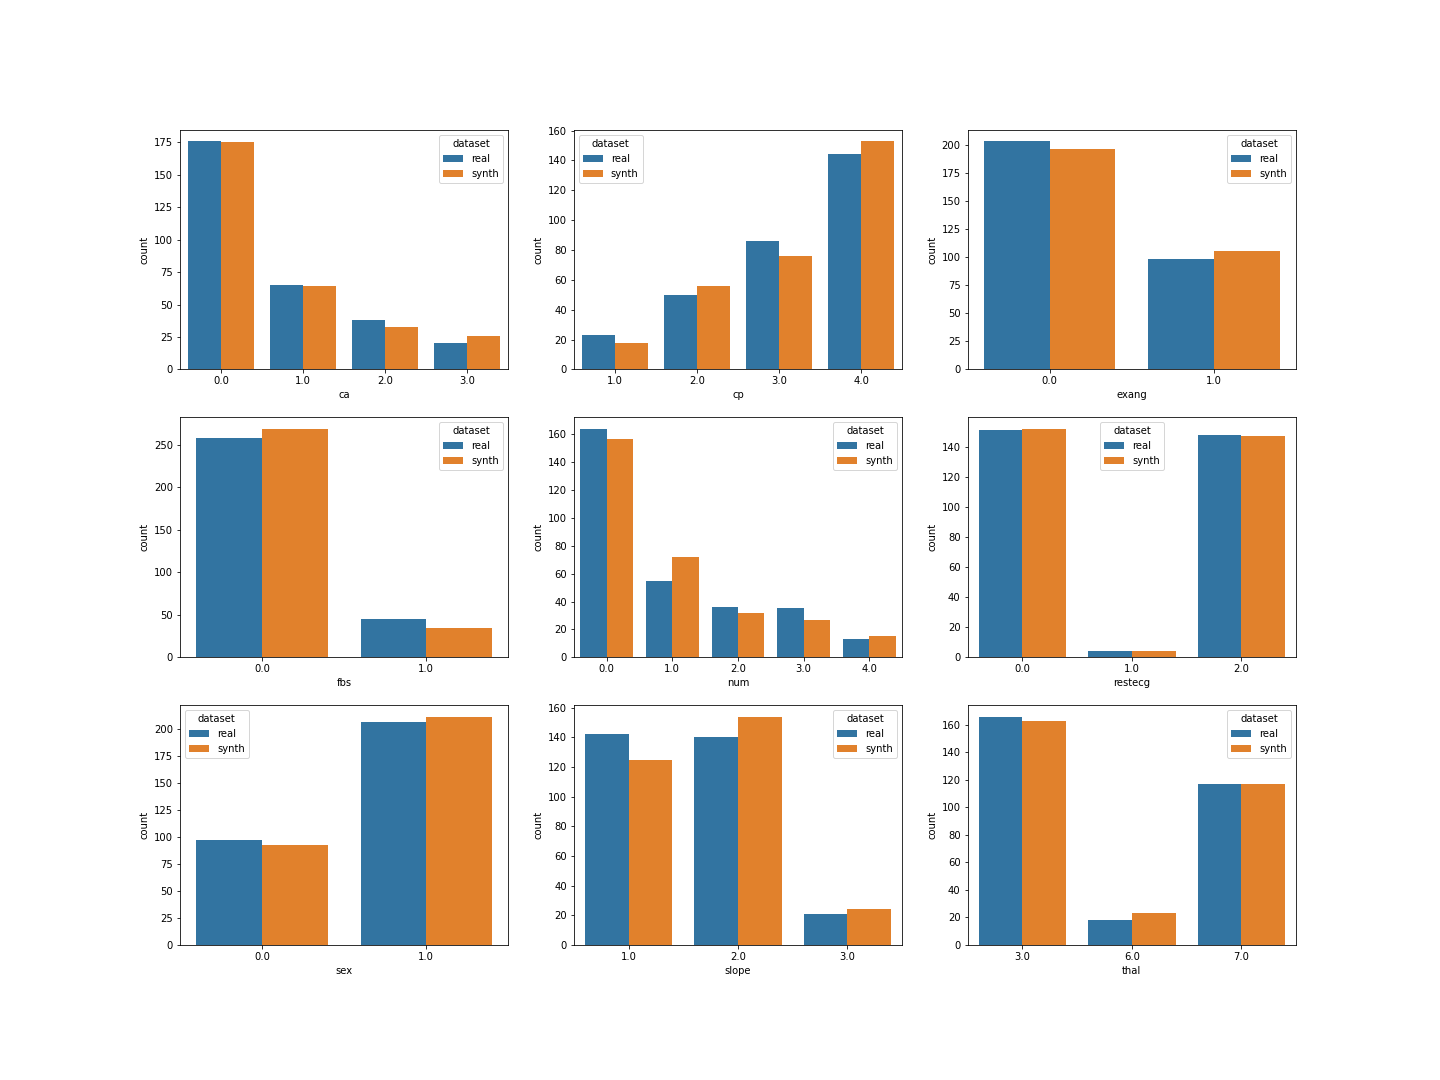
\includegraphics[scale=0.23]{figures/cat.png}
    \caption{Categorical Variables plotted}
    \label{fig:catgorical}
\end{figure}

\begin{figure}[t]
    \centering
    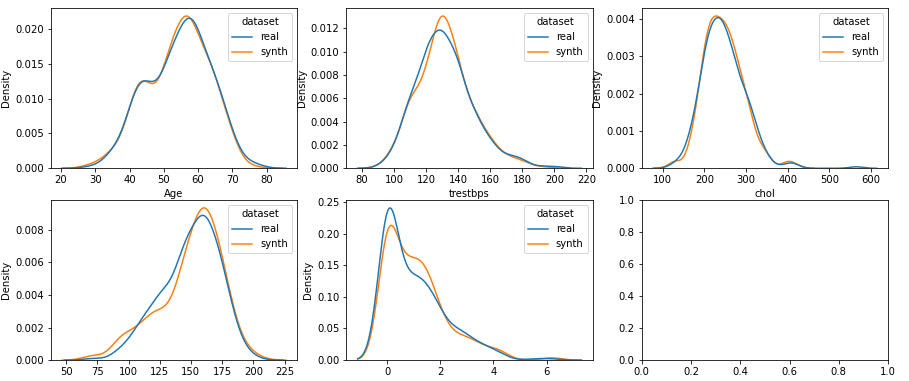
\includegraphics[width=\textwidth]{figures/continuous_plot_0.png}
    \caption{Continuous Variables plotted}
    \label{fig:continuous}
\end{figure}



\subsection{Discussion \& Conclusion}

The data possible to create to evaluate similarities between two datasets is important not only for synthetic vs real datasets. For example, in distributed learning, where different silos exist, with similar or even equal features, a method for evaluating the similarities can be useful for understanding how the populations are similar between them, trying to shed light on the most similarities among them, or different in order to understand the differences in the silos or data acquisition inside them.
Furthermore, the differences can be assessed on a more granular level. The column-wise similarities can be different from the inter-column similarities and this in itself, can be a metric of interest regarding the quality of the synthetic data and its generator.

With this work, we hope to help institutions and academics get access to a benchmark of the datasets provided in order to leverage synthetic data in the healthcare space. Finally, we hope this work helps other researchers reach an evaluation metric that could be a unique and clear response to the question of how similar two datasets are.




\section{Can We Use Machine Learning Feature to Compare Datasets?}\label{subsec:similarity}
This section is based on the paper entitled "Using Machine Learning Models' feature importance to assess dataset similarity". The reasoning behind this paper was the results of section \ref{subsec:gans}, where we felt that evaluation metrics for synthetic data could be improved. Better yet, we felt that the comparison of two datasets (that shared the same columns) could be done in a more robust way. Being that the current gold-standard was cross-validation which was not bound to any number range and the significance of the result could not be easily interpretable. We used the feature importance of several \ac{ml} models to compare datasets and concluded that it was a valid alternative to the traditional metrics.

\subsection{Introduction}
In recent years, the use of \ac{ai} and \ac{ml} algorithms has gained increasing prominence in healthcare research and practice. One of the key requirements for the successful application of these methods is access to large, high-quality datasets. However, in many cases, the availability of such datasets can be limited due to issues around data privacy, security, and ethical concerns \cite{chingOpportunitiesObstaclesDeep2018a}. To address this challenge, synthetic data has emerged as a promising solution. Synthetic data refers to artificially generated data that closely mimic the statistical properties and patterns of real-world data \cite{mullerEvaluationSyntheticElectronic2022}.

Synthetic data has the potential to overcome many of the limitations associated with real-world data, such as the lack of sufficient data volume, noise, and privacy concerns. Even though there are still doubts if the privacy part is the silver bullet sometimes referred to \cite{stadlerSyntheticDataPrivacy2020}, the upsampling part is a standard use for years now. However, the quality of synthetic data generated by various techniques can vary significantly, and it is essential to assess the quality of synthetic data before its usage. In healthcare, the assessment of synthetic data is crucial to ensure that it can provide valid insights and inform decision-making processes.

The assessment of synthetic data in healthcare is essential for its successful use in various applications, such as developing predictive models, testing algorithms, and conducting clinical trials. The use of synthetic data can significantly enhance the efficiency and effectiveness of healthcare research and practice. However, it is crucial to ensure that the synthetic data used in these applications are of high quality and validated to provide reliable and valid insights. The evaluation of synthetic data quality involves comparing its statistical properties and patterns with those of the original data. We can assess how similar columns are to each other through several statistical tests, and then we can infer some inter-column properties with methods like cross-validation, where two datasets are split into train tests and cross-tested and then the ratio between the evaluation result of both datasets is used as a metric.\cite{mullerEvaluationSyntheticElectronic2022,goncalvesGenerationEvaluationSynthetic2020a}. However, this methodology is a big proxy for such an inter-column relationship. Can we try to provide a better metric than this one to evaluate how similar are the inter-column relationship of two distinct datasets? In this paper, we suggest using feature importance values to create a more explainable and reasonable metric for inter-column relationships.

\subsection{Rationale and Related Work}
% !TeX root = ../../thesis.tex

Recently there has been a series of works related to assessing how synthetic data generators behave with data like the work of Emam et al. \cite{emamUtilityMetricsEvaluating2022} that especially focused on utility metrics for synthetic data generators. At the moment, comparing data is based on intra-columns and inter-columns relationship. The intracolumn relationship is assumed as something that compares equal columns between datasets, with highly known statistical methods like chi-squared or \ac{ks} like done in the works of \cite{combrinkComparingSyntheticTabular2022} among many others, acting more like sanity checks than anything else. 
Other known metrics are distance-based metrics like \ac{jsd}, Wasserstein Distance, Bhattacharyya Distance or Hellinger distance, which are based on the calculation of the distance between distributions like seen in the works of several teams \cite{ISI:000557358500024,choiGeneratingMultilabelDiscrete2017,Baowaly2019}.

However, regarding inter-column relationships, the metrics applied are often very different across papers. One example of trying to capture inter-column relationship is about the use of propensity score \cite{rosenbaumCentralRolePropensity1983,mullerEvaluationSyntheticElectronic2022} where a classifier is trained to the merged datasets, with the added variable of the original dataset (i.e., 1 for real and 0 for synthetic). The model is trained and the propensity Mean square error is the  mean squared difference of the estimated probability from the average prediction
Most recently, a unified metric appeared as the sum of other metrics known as described in the work of Chundawat et al., \cite{chundawatTabSynDexUniversalMetric2022}, known as TabSynDex. Other examples are likelihood of fitness like in the works of \cite{xuModelingTabularData2019b}, coverage support \cite{goncalvesGenerationEvaluationSynthetic2020a} or very specific metrics implemented for evaluating specific data generators.
However, the most used metric is cross-validation, which takes two datasets, one that is real and a second which is synthetic and we split both into train and test and train a machine learning model on the real data training set, then we test the model on both test sets. Then a ratio is created, rendering the actual value. This methodology, even if gold-standard at the moment for this type of study, has some liabilities since this value can be a bit erratic, and even above one since the evaluation metric could be better on the second dataset and we don't have a clear grasp of what that can represent in terms of dataset similarity. The image \ref{fig:1} represents this in detail. Several works used this metric as the comparing metric \cite{mullerEvaluationSyntheticElectronic2022}.

%TC:ignore
\begin{figure}[tbph]
\centering
\caption{Cross-Validation of datasets}\label{fig:1} 
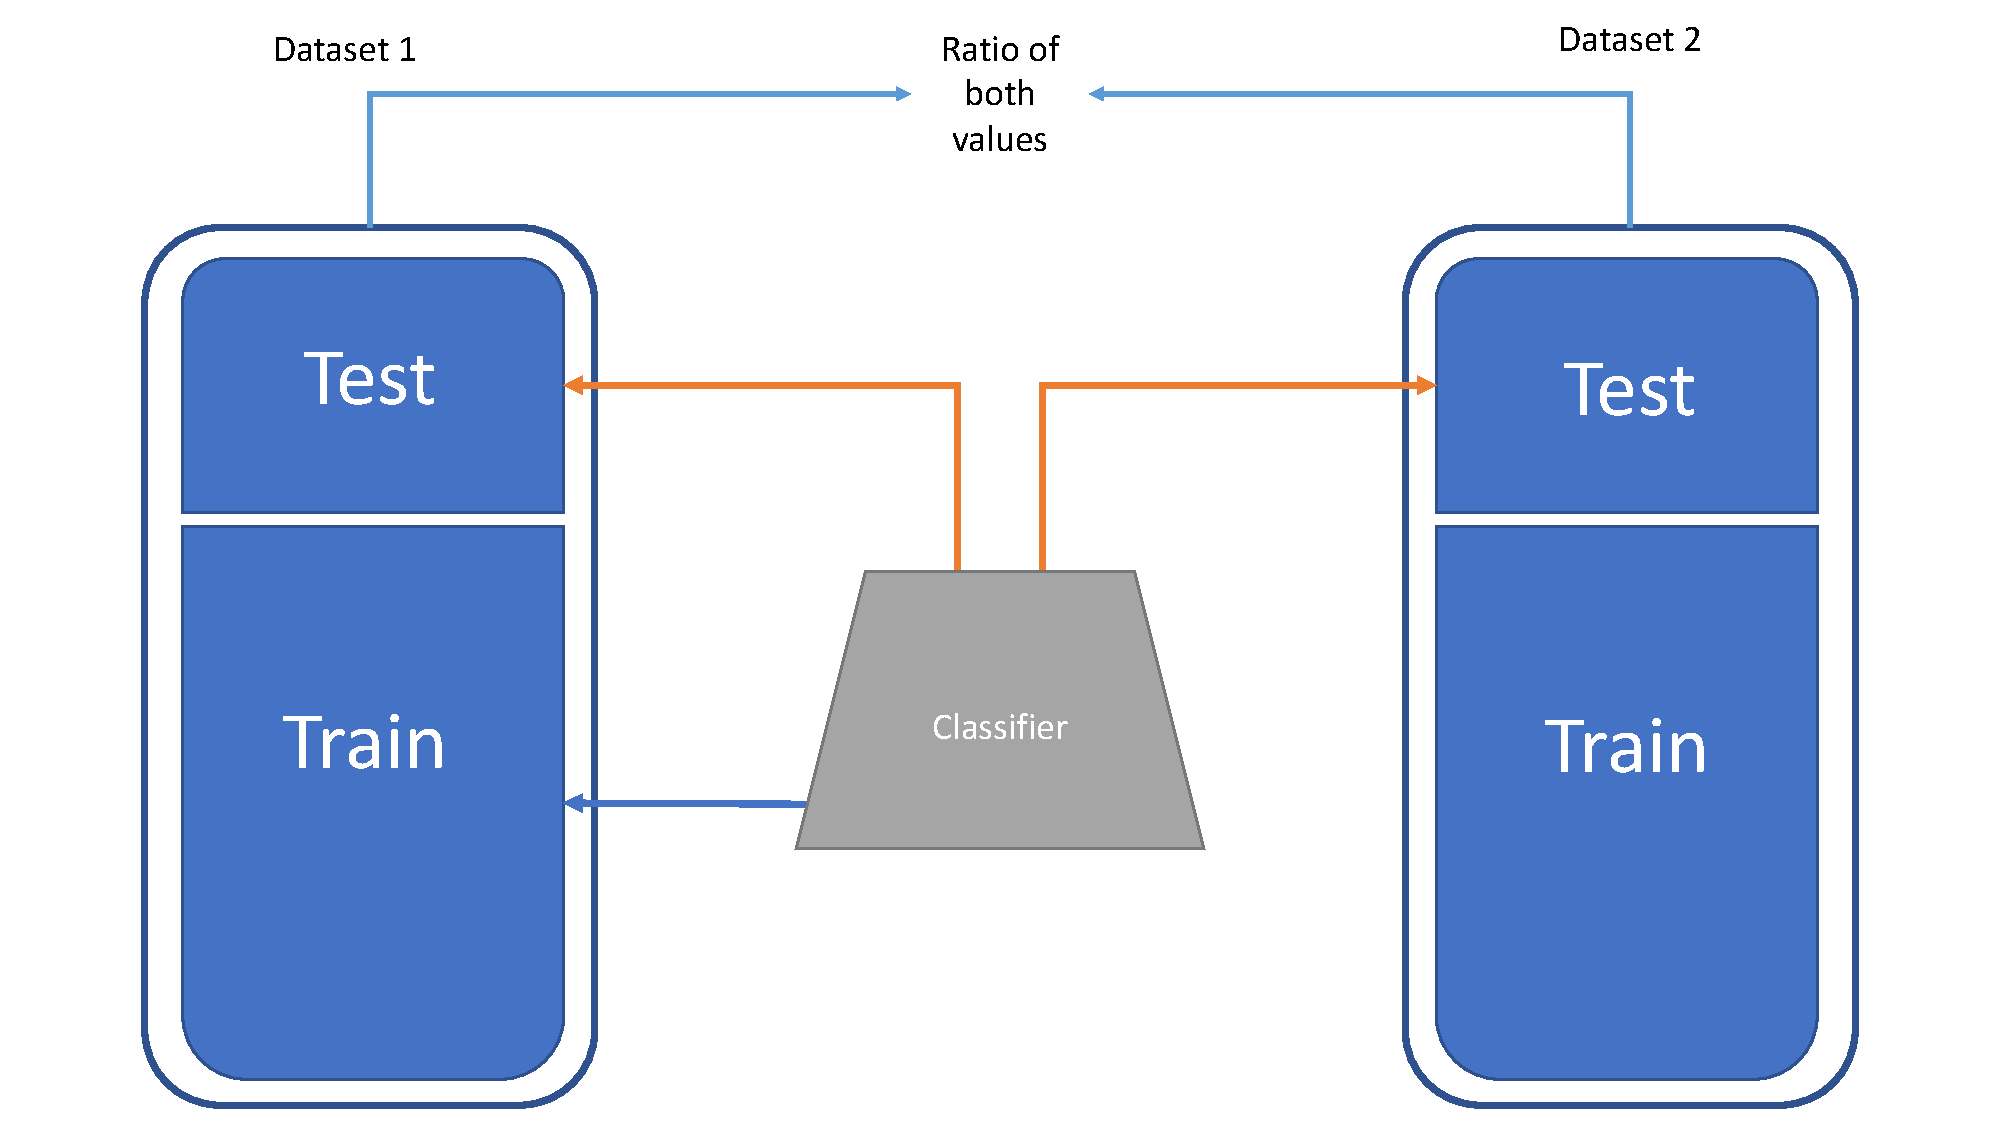
\includegraphics[scale=0.35]{figures/imagem1.pdf}
\end{figure}
%TC:endignore




%Utility Metrics for Evaluating Synthetic Health Data Generation Methods: Validation Study



\subsection{Materials \& Methods}
\subsubsection{Materials}
% !TeX root = ../../thesis.tex


We used 5 datasets from the UCI dataset repository. The ones chosen were related to healthcare and were heart disease \cite{misc_heart_disease_45}, thyroid disease \cite{misc_thyroid_disease_102}, liver disorders \cite{misc_liver_disorders_60}, breast cancer \cite{misc_breast_cancer_wisconsin_diagnostic_17} and the primary tumour dataset \cite{misc_primary_tumor_83}. These datasets were chosen due to three main reasons: 1) being open and facilitating recreation of results; 2) being tabular with mixed datatypes to better represent data in the real world and 3) diversity across domains inside healthcare (different diseases and contexts).

We made minimal preprocessing on the datasets, namely removing the missing variables by imputing the mean on continuous variables and mode on categorical.
We also created several synthetic datasets by applying known methods. Descriptive statistics of the datasets used are shown in table \ref{tab:descrptive_feature}.
\begin{small}    
\begin{table}[htpb]
    \footnotesize
        \caption{Descriptive statistics of datasets used. Mean (Standard Deviation) for continuous variables. Mode [nr categories] for categorical variables.}\label{tab:descrptive_feature}
            \begin{tabularx}{\textwidth}{lXll|lXll}
                \toprule
            Dataset & Column                         & Statistic    & \% Nulls & Dataset & Column          & Statistic    & \% Nulls \\
            \midrule
            heart   & Age                            & 54.4 (9.0)   & 0.0      & liver   & gammagt         & 38.3 (39.3)  & 0.0      \\
            heart   & sex                            & 1.0 {[}2{]}  & 0.0      & liver   & drinks          & 3.5 (3.3)    & 0.0      \\
            heart   & cp                             & 4.0 {[}4{]}  & 0.0      & liver   & Selector        & 2 {[}2{]}    & 0.0      \\
            heart   & trestbps                       & 131.7 (17.6) & 0.0      & thyroid & Class           & 1 {[}3{]}    & 0.0      \\
            heart   & chol                           & 246.7 (51.8) & 0.0      & thyroid & T3              & 109.6 (13.1) & 0.0      \\
            heart   & fbs                            & 0.0 {[}2{]}  & 0.0      & thyroid & TST             & 9.8 (4.7)    & 0.0      \\
            heart   & restecg                        & 0.0 {[}3{]}  & 0.0      & thyroid & TSTRI           & 2.1 (1.4)    & 0.0      \\
            heart   & thalach                        & 149.6 (22.9) & 0.0      & thyroid & TSH             & 2.9 (6.1)    & 0.0      \\
            heart   & exang                          & 0.0 {[}2{]}  & 0.0      & thyroid & TMAX            & 4.2 (8.1)    & 0.0      \\
            heart   & oldpeak                        & 1.0 (1.2)    & 0.0      & tumour   & class           & 1 {[}21{]}   & 0.0      \\
            heart   & slope                          & 1.0 {[}3{]}  & 0.0      & tumour   & age             & 2 {[}3{]}    & 0.0      \\
            heart   & ca                             & 0.0 {[}4{]}  & 1.3      & tumour   & sex             & 2 {[}2{]}    & 0.3      \\
            heart   & thal                           & 3.0 {[}3{]}  & 0.7      & tumour   & histologic-type & 2 {[}3{]}    & 19.8     \\
            heart   & num                            & 0 {[}5{]}    & 0.0      & tumour   & degree-of-diffe & 3 {[}3{]}    & 45.7     \\
            breast  & Clump Thickness               & 4.4 (2.8)    & 0.0      & tumour   & bone            & 2 {[}2{]}    & 0.0      \\
            breast  & Uniformity of Cell Size     & 3.1 (3.1)    & 0.0      & tumour   & bone-marrow     & 2 {[}2{]}    & 0.0      \\
            breast  & Uniformity of Cell Shape    & 3.2 (3.0)    & 0.0      & tumour   & lung            & 2 {[}2{]}    & 0.0      \\
            breast  & Marginal Adhesion             & 2.8 (2.9)    & 0.0      & tumour   & pleura          & 2 {[}2{]}    & 0.0      \\
            breast  & Single Epithelial Cell Size & 3.2 (2.2)    & 0.0      & tumour   & peritoneum      & 2 {[}2{]}    & 0.0      \\
            breast  & Bare Nuclei                   & 3.5 (3.6)    & 2.3      & tumour   & liver           & 2 {[}2{]}    & 0.0      \\
            breast  & Bland Chromatin               & 3.4 (2.4)    & 0.0      & tumour   & brain           & 2 {[}2{]}    & 0.0      \\
            breast  & Normal Nucleoli               & 2.9 (3.1)    & 0.0      & tumour   & skin            & 2 {[}2{]}    & 0.3      \\
            breast  & Mitoses                        & 1.6 (1.7)    & 0.0      & tumour   & neck            & 2 {[}2{]}    & 0.0      \\
            breast  & Class                          & 2 {[}2{]}    & 0.0      & tumour   & supraclavicular & 2 {[}2{]}    & 0.0      \\
            liver   & mcv                            & 90.2 (4.4)   & 0.0      & tumour   & axillar         & 2 {[}2{]}    & 0.3      \\
            liver   & alkphos                        & 69.9 (18.3)  & 0.0      & tumour   & mediastinum     & 2 {[}2{]}    & 0.0      \\
            liver   & sgpt                           & 30.4 (19.5)  & 0.0      & tumour   & abdominal       & 2 {[}2{]}    & 0.0      \\
            liver   & sgot                           & 24.6 (10.1)  & 0.0      &         &                 &              &          \\
              \bottomrule
            \end{tabularx}

        \end{table}
    \end{small}



\subsubsection{Method Overview}
For this work, our goal is to test several metrics based on the ranking of feature importance of a trained model. Normalized Discounted Cumulative Gain (NDCG) \cite{wangTheoreticalAnalysisNDCG} which is the sum of the true scores ranked in the order induced by the predicted scores, after applying a logarithmic discount. Then divide by the best possible score to obtain a score between 0 and 1. It is calculated by
\begin{equation}
\text{{NDGC}} = \frac{{\text{{DCG}}(P)}}{{\text{{IDCG}}(P)}}
\end{equation}
where $\text{{DCG}}(P)$ is the Discounted Cumulative Gain and $\text{{IDCG}}(P)$ is the Ideal Discounted Cumulative Gain. 

Cohen's kappa coefficient \cite{doi:10.1177/001316446002000104}  is a statistic that is commonly used to assess the level of agreement between two or more raters or evaluators who are providing categorical ratings or rankings of a set of items. So, we want to use to assess if it could be of use to check how similar the ranking of the features is, using the numbers as categorical.
\begin{equation}
\kappa = \frac{{P_o - P_e}}{{1 - P_e}}
\end{equation}

where \(P_o\) is the observed agreement between the two raters and \(P_e\) is the expected agreement between the two raters by chance.

We also intend to use the $R^2$ to check if the explainability changes across datasets.
\begin{equation}
R^2 = 1 - \frac{{\sum_{i=1}^n (y_i - \hat{y}_i)^2}}{{\sum_{i=1}^n (y_i - \bar{y})^2}}
\end{equation}


where \(y_i\) are the observed values of the dependent variable, \(\hat{y}_i\) are the predicted values of the dependent variable, \(\bar{y}\) is the mean of the observed values of the dependent variable and \(n\) is the number of data points.

Then we intend to use ranking metrics, namely Kendall tau, weighted Kendall tau and RBO.
Kendall tau is a measure of correlation that measures the similarity between two rankings. It is commonly used in statistics and data analysis to evaluate the agreement or disagreement between two sets of rankings.

The Kendall tau coefficient \cite{kendallTreatmentTiesRanking1945} is defined as the difference between the number of concordant and discordant pairs of observations, divided by the total number of pairs. A concordant pair is a pair of observations that have the same ranking order in both sets, while a discordant pair is a pair of observations that have opposite ranking orders. The Kendall tau coefficient ranges from -1 to 1, where -1 represents perfect negative correlation, 0 represents no correlation, and 1 represents perfect positive correlation. 
\begin{equation}
\tau = \frac{{\text{{number of concordant pairs}} - \text{{number of discordant pairs}}}}{{\text{{total number of pairs}}}}
\end{equation}

Weighted Kendall tau  \cite{vignaWeightedCorrelationIndex2015} is an extension of Kendall tau that takes into account the importance or weight of each observation in the rankings. In some cases, some observations may be more important than others, and their positions in the ranking may have a greater impact on the overall correlation. Weighted Kendall tau assigns a weight to each observation, and the correlation is calculated based on the weighted concordant and discordant pairs.
\begin{equation}
\tau_w = \frac{{\sum_{i<j} w_{ij} \cdot sgn(x_i - x_j)}}{{\sum_{i<j} w_{ij}}}
\end{equation}

where $w_{ij}$ is the weight associated with the pair $(x_i, x_j)$ and $sgn(\cdot)$ is the sign function.
Rank-biased overlap (RBO) \cite{webberSimilarityMeasureIndefinite2010} is a measure of similarity between two ranked lists or rankings. It takes into account the order of items in the two lists, and it can be used to evaluate the quality of search results, recommendations, or any other kind of ranked list it has been shown to be more robust and accurate than other similarities measures such as Kendall tau or Spearman's rank correlation coefficient. 
\begin{equation}
\text{{RBO}} = (1 - \rho) \cdot \sum_{d=1}^{\infty} \left( \frac{{g_d}}{{d}} \right) \cdot \rho^d
\end{equation}

where $\rho$ is the weight, $g_d$ is the gain at depth $d$, and $\sum_{d=1}^{\infty}$ indicates the summation over all depths.


Finally, we intend to use text-distance metrics. The theory behind this experiment is to treat the ordered columns in a ranking manner and apply text-distance metrics to check the distance between the two. Levenshtein distance \cite{navarroGuidedTourApproximate2001} is the minimum number of single-character insertions, deletions, or substitutions required to transform one string into another. Damerau-Levenshtein distance \cite{navarroGuidedTourApproximate2001} is similar to Levenshtein distance but also includes the transposition of two adjacent characters as an allowable operation. The hamming distance \cite{6772729} is a measure of the difference between two strings of equal length, defined as the number of positions at which the corresponding symbols are different. Jaro-Winkler distance \cite{navarroGuidedTourApproximate2001} is a string similarity measure that takes into account the number of matching characters, the number of transpositions, and the length of common prefixes, with a higher weight given to the common prefix.




\begin{algorithm}[hbtp]
\SetAlgoLined

\For {i in number of columns to test}{
\For {rep in  10 repetitions}{ 
permutate values in i columns

\For {dataset in dataset pair}{

\For {target in dataset columns}{

Train-Test Split (95:5)
 model fit to train
     get feature importance per column
     Create an ordered rank of features 
 }}}}


 \caption{Testing similarity scores in tabular datasets}
 \label{alg:simil_1}

\end{algorithm}



The algorithms chosen were decision trees, random forests, \ac{svm},  \ac{knn}, and linear regression/logistic regression as implemented in the \textit{scikit-learn} package \cite{scikit-learn}. The text distance metrics were implemented by the text-distance package \cite{orsiniumTextdistanceComputeDistance}. Kendall tau, weighted Kendall tau were used as implemented by scipy \cite{virtanenSciPyFundamentalAlgorithms2020a} and RBO, as implemented in \cite{chenRankbiasedOverlapRBO2023}.








\subsection{Results}
With the method described in the algorithm \ref{alg:simil_1}, we created a figure where the metrics are presented with increasingly different datasets: figure \ref{fig:lineplot}.
%Then we compared the difference in the metric across iterations, rendering figure \ref{fig:boxplot}.


%TC:ignore
\begin{figure}[htbp]
\centering
\caption[Plot showing the decrease of the metric over increasingly changed datasets.]{Plot showing the decrease of the metric over increasingly changed datasets. The X axis represents the number of columns mutated. The Y axis represents the value of the metric and the hue represents the algorithm used to calculate the metric.}\label{fig:lineplot} 
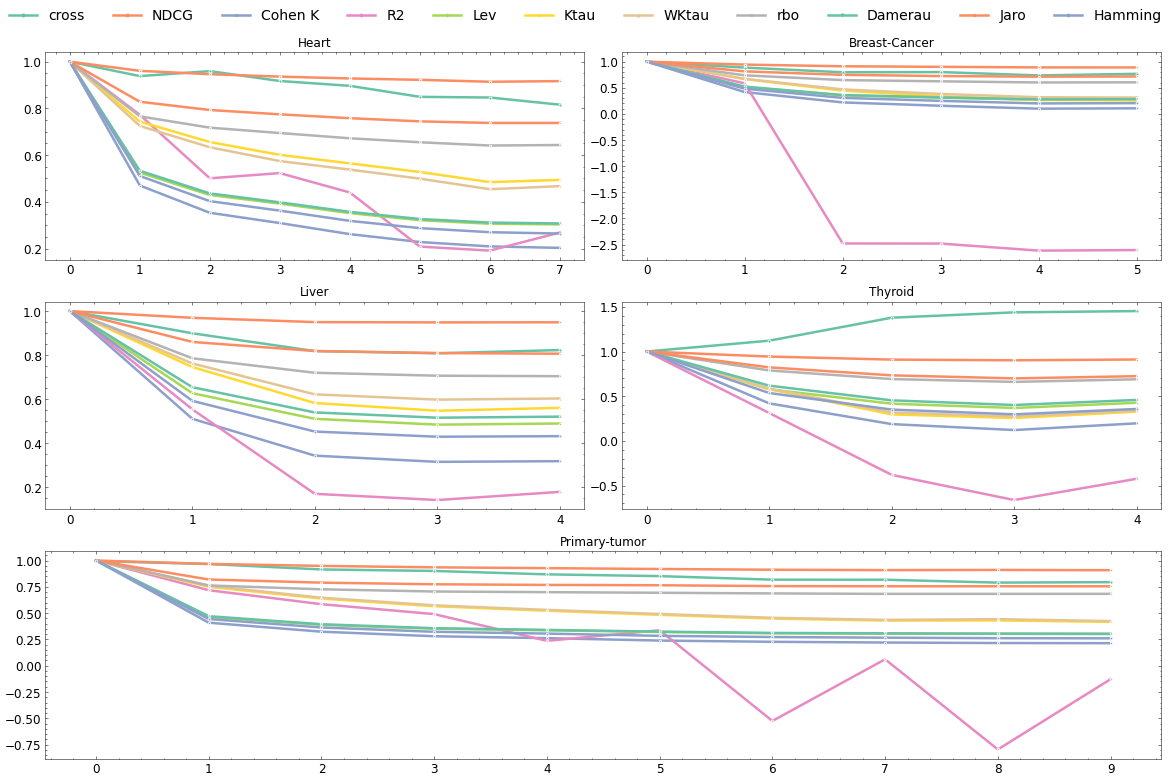
\includegraphics[scale=0.37]{figures/multiple_datasets.png}
\end{figure}
%TC:endignore


%TC:ignore
\begin{figure}[htbp]
\centering
\caption{Plot showing the values at 50\% columns mutated across all datasets and algorithms per metric type}\label{fig:boxplot} 
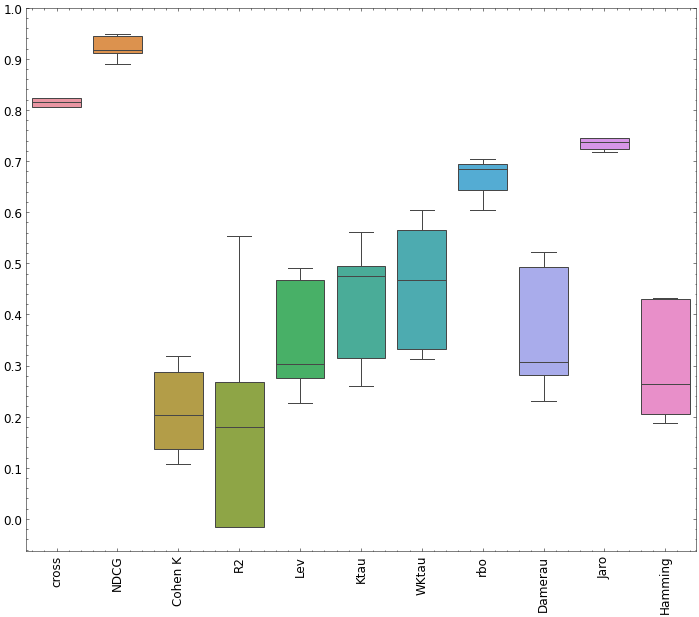
\includegraphics[scale=0.55]{figures/50_percent_data.png}
\end{figure}
%TC:endignore


The number of repetitions and how that impacts the variance of the scores is shown in figure \ref{fig:facet_plot}.






%TC:ignore
\begin{figure}[htbp]
\centering
\caption{Plot the variance of different repetitions for every metric and the number of different columns changed. X is the number of columns mutated. Colour is the number of repetitions for each mutation and Y is the variance of the data. }\label{fig:facet_plot} 
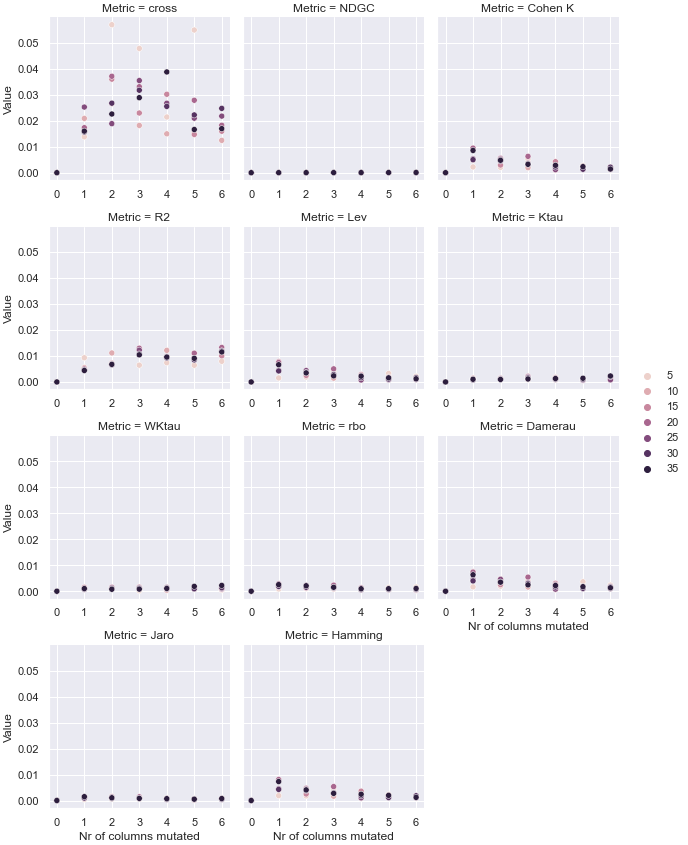
\includegraphics[scale=0.55]{figures/facet_plot.png}
\end{figure}
%TC:endignore

As for the test for the synthetic and real datasets, the results are displayed in figure \ref{fig:synth_result}.
%TC:ignore
\begin{figure}[htbp]
\centering
\caption{Result on a synthetic and real data }\label{fig:synth_result} 
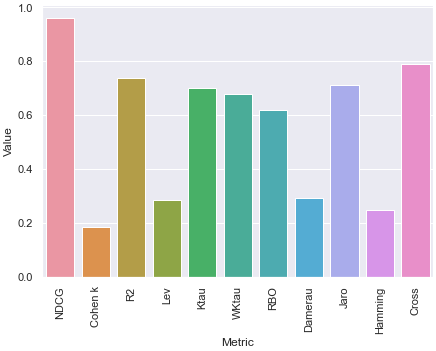
\includegraphics[scale=0.65]{figures/synthetic.png}
\end{figure}
%TC:endignore
\subsection{Discussion}
% !TeX root = ../../thesis.tex


With the results found, we feel that are better alternatives to CC. \ac{rbo} seems like alternatives to CC. Firstly, as with Kendall tau and Weighted Kendall tau, it seems to be directly connected to a difference in the dataset. They seem to lower from 1 (equal datasets) to around 50\% when the columns changed are half of the columns of the dataset, which seems an encouraging result. Secondly, it is a bounded metric between 0 and 1, which is helpful for interpretation since, as we have seen with for example CC and $R^2$, they can go outside these bounds, making  the interpretation of the results more difficult for these scenarios. Thirdly, variance across different iterations is also lower. Even though the variance across all metrics is quite low (except $R^2$), \ac{rbo} seems to have less variance than Kendall tau and Weighted Kendall tau, which could be the differentiating factor between these 3 metrics.  With CC, we have a variance that despite low (on the 0.01 level), is still higher than the other metrics (except $R^2$) which have variance around 0. This is important, since it is independent of numbers of runs to get a stable result.
Regarding text metrics, they have a drastic drop with only one column mutated (Figure~\ref{fig:lineplot}) but the decrease is steady afterwards. As for $R^2$, we see that it is not a good metric for this type of problem, since it is not bounded between 0 and 1, and it has a high variance across different iterations. This is probably due to the fact that it is a regression metric, and it is not designed for this type of problem.

While the proposed metrics such as \ac{rbo} and Kendall Tau have shown promise in capturing changes in feature importance, there are several limitations that should be addressed in future research. 
Firstly, the possibility of synthetic datasets may be different in other ways that a value permutation could not grasp. For example, the distribution of the data could be different, or the number of unique values could be different. Nevertheless, we tested with 3 sets of synthetic datasets produced by us as counterpart to the 5 original datasets to make at least a sanity check that the new approaches assessed are at least in tune with CC for actual synthetic datasets (Figure~\ref{fig:synth_result} and \ref{fig:synth_heat}). We can see that the values are at least near the values of CC. Moreover, they seem to have less variability, which can make sense taken into account the synthetic data generator was the same. These results also point towards the direction that these new approaches could be a good alternative to CC.

Secondly, the metrics have primarily been tested on synthetic datasets, and their performance on real-world datasets with varying distributions, noise, and missing data remains to be fully explored. Thirdly, these metrics may not fully account for complex interactions between features, which are often present in real-world datasets. Future work could focus on incorporating feature interaction measures or combining these metrics with statistical distance metrics to better reflect such complexities. Additionally, while the variance of the proposed metrics is generally low, exploring methods to further reduce variance, especially in high-dimensional datasets, would enhance their robustness. Finally, future research could develop methods to provide confidence intervals or uncertainty estimates for these metrics, which would improve their interpretability and reliability in practical applications.


With these findings, we believe that progress has been made in comparing tabular datasets, which may prove beneficial not only for evaluating synthetic data generators but also for formalizing the degree of similarity between datasets that share common features. This approach provides a valuable reference for the development of new data generators and enhances confidence in benchmarks and comparisons.
\subsection{Conclusion}
% !TeX root = ../../thesis.tex

Comparing two tabular datasets has been growing in demand in the past year mainly because of the increase in popularity of tabular data synthesis methods which have exhibited the potential in generating valuable synthetic data. However, due to the absence of a uniform metric, evaluating different methods has been inconsistent. This research proposes some alternatives for assessing synthetic tabular data's utility. \ac{rbo} seems to have the potential to capture inter-column relationships in a more consistent way than cross-classification. They could become a useful tool for comparing statistical methods of generating synthetic tabular data. Furthermore, this metric can aid in evaluating these generators' training, providing insights into improving synthetic data quality. The proposed metrics open up possibilities for future research to enhance tabular data synthesis methods and compare two datasets overall. Future research could be expanded in new comparison with others evaluation metrics, other datasets and other synthetic data generators.


\section{Can We Use Machine Learning to Create Automatic Data Quality Assessments?}\label{subsec:dq}
This section is based on the paper entitled "Development and Validation of a Data Quality Evaluation Tool in Obstetrics Real-World Data through \ac{hl7} \ac{fhir} interoperable Bayesian Networks and Expert Rules" This paper focuses on the fact that data quality is a major concern in healthcare. We developed a tool that could be used to assess the quality of data in a \ac{ehr} and provide a report on the quality of the data. We used a combination of \ac{bn} and expert rules to assess the quality of the data. Furthermore, we tested the tool on 9 real-world datasets of obstetrics \acp{ehr} and concluded that the tool was a valid alternative to the traditional methods of assessing data quality.
%\input{chapters/data-quality-paper}
\subsection{Introduction}
With the wide spreading of healthcare information systems across all contexts of healthcare practice, the production of health-related data has followed this incremental behaviour. The potential for using this data to create new clinical knowledge and push medicine further is tempting \cite{martin-sanchezBigDataMedicine2014}.
However, to correctly use the data stored in \acp{ehr}, the quality of the data must be robust enough to sustain the clinical decisions made based on this data. Data quality cannot be construed as a linear concept; it is intrinsically dependent on the context in which it is evaluated. The quality thresholds and dimensions required to classify the quality of the data depend on the purpose that we intend to use that very same data \cite{waljiElectronicHealthRecords2019}. These uses can be very distinct and have different impacts as well. For one, we can use data to support day-to-day decisions regarding individual patients’ care \cite{verheijPossibleSourcesBias2018}. These decisions can include ones based on recorded information to understand a patient’s history, clinical decision support systems based on this data, or even using the data to help support a more macro, public health-oriented decision. Another area is using information for management purposes. The data can be used by management bodies and regulatory authorities to extract metrics regarding the quality of care or reimbursement purposes. Thirdly, data can be used for research purposes, namely observational studies and, more recently, to support clinical trials through real-world evidence analysis \cite{coreyAssessingQualitySurgical2020,verheijPossibleSourcesBias2018,wengClinicalDataQuality2020}. 
So, all the \ac{ehr} data-based decisions can only be as good as the data supporting them. Several studies have already warned about the lack of data quality in \acp{ehr} and how this can be a significant hurdle to an accurate representation of the population and potentially lead to erroneous healthcare decisions \cite{reimerDataQualityAssessment2016a,joukesImpactElectronicPaperBased2019a,huserMultisiteEvaluationData2016,zhangUnderstandingDetectingDefects2020,kramerImpactDataQuality2021,gigantiImpactDataQuality2019}.

There are several steps in the data lifecycle that can be prone to error, from data generation, where the data is registered by healthcare professionals, passing by data processing, whether inside healthcare institutions or by software engineers aiming to reuse data, to data interpretation and reuse, where investigators
try to interpret the meaning of registered data\cite{wengClinicalDataQuality2020}.
So, with all of the data’s possible uses added to the several steps that can introduce errors throughout the data lifecycle, data quality frameworks and sequential implementations can have very distinct approaches and methodologies to assess data quality. Data quality tools for checking data being registered live to support day-to-day decisions will be significantly different from one whose only purpose is to provide quality checks for research purposes. So, methodologies to tackle these issues are necessary for guaranteeing the quality of healthcare practice and the knowledge derived from \ac{ehr} data. Consequently, in this paper, we propose:
\begin{myitemize}
    \item Create a tool for identifying data quality issues in obstetrics \acp{ehr};
    \item Enlighten on the issues that can appear with a full deployment of such a tool
    \item Suggestion of a creation of a single score for data quality for comparison of high-quality and low-quality records in a database.
    \item Assess how such a tool can work in early-stage real-world scenarios and how to work with obstetricians to improve data quality.
    \item Identify data quality issues on obstetrics data
\end{myitemize}


%Data quality is a crucial aspect of the healthcare industry, as it impacts the accuracy of diagnoses, treatment plans, and patient outcomes. The reliability and accuracy of healthcare data have far-reaching consequences, including financial implications, patient safety, and legal ramifications. Inaccurate or incomplete data can lead to incorrect diagnoses, inappropriate treatments, and ultimately harm to patients. Therefore, ensuring the quality of healthcare data is essential to providing effective and safe healthcare services.

%One of the main reasons why data quality is so critical in healthcare is that healthcare data is often used to make important decisions, such as treatment plans, patient management, and resource allocation. Inaccurate or incomplete data can lead to misdiagnosis, inappropriate treatment, and increased healthcare costs. Furthermore, inaccurate data can hinder research efforts and impede the development of new treatments and therapies.

%Another key aspect of data quality in healthcare is its role in patient safety. Accurate and reliable data is essential for ensuring patient safety, particularly in areas such as medication management, clinical decision-making, and adverse event reporting. Poor data quality can lead to medication errors, adverse drug reactions, and other types of harm to patients.

%Finally, data quality is also important for legal and regulatory compliance in healthcare. Accurate and complete data is required for compliance with regulations such as HIPAA, the Affordable Care Act, and other regulatory requirements. Poor data quality can result in legal and financial penalties, as well as reputational damage for healthcare organizations.

%Overall, data quality is a crucial aspect of healthcare, with far-reaching implications for patient safety, healthcare costs, and regulatory compliance. Ensuring the quality of healthcare data requires a comprehensive approach that includes data governance, data management, data quality assurance, and ongoing monitoring and improvement efforts. By prioritizing data quality, healthcare organizations can provide better patient care, improve outcomes, and reduce costs.





\subsection{Background and Related Work}
There is already a significant number of papers trying to define data quality assessment frameworks for \ac{ehr} data, all of them plausible and recommendable, already described in other papers \cite{bianAssessingPracticeData2020}. The literature has over 20 different methods, descriptions, and summaries of  different frameworks over the years. Some may be highlighted from the review from Weiskopf et. al, \cite{weiskopfMethodsDimensionsElectronic2013}, where five data quality concepts were identified over 230 papers: Completeness, Correctness, Concordance, Plausibility and Currency. 



The work of Saez et al. defined a unified set of \ac{dq} dimensions: completeness, consistency, duplicity, correctness, timeliness, spatial stability, contextualization, predictive value, and reliability \cite{saezOrganizingDataQuality2012}. Then a review of Bian et al. \cite{bianAssessingPracticeData2020} expanded on the previous ones, categorizing data quality into 14 dimensions and mapping them to the previous most known definitions. These were: currency, correctness, plausibility, completeness, concordance, comparability, conformance, flexibility, relevance, usability, security, information loss, consistency, and interpretability.

Finally, the work of Khan et al. tried to harmonize data quality assessment frameworks, which simplified all previous concepts into three main categories: Conformance, Completeness and Plausibility and two assessment contexts: Verification and Validation \cite{kahnHarmonizedDataQuality2016a}.
Despite all of these comprehensive works, there is still no consensus regarding which one is best or which has taken the lead in usage. Moreover, looking at all of the descriptions related in the literature, a significant portion of concepts are overlapping, and sometimes hard to conceptualize such dimensions in practice.

As for implementations, there are already some available, such as the work from \cite{phanAutomatedDataCleaning2020} where a tool created by primary care in the Flanders was built to assess completeness and percentage of values within the normal range.
The work from Liaw et al. \cite{liawQualityAssessmentRealworld2021} already reviewed some data quality assessment tools, like tools from OHDSI \cite{hripcsakObservationalHealthData2015} or TAQIH \cite{alvarezsanchezTAQIHToolTabular2019}. 
Additionally, we found some others with similar purposes and characteristics like the work presented data dataquieR \cite{schmidtFacilitatingHarmonizedData2021}, an R language-based package that can assess several data quality dimensions in observational health research data. 
Also, the work from Razzaghi et al. developed a methodology for assessing data quality in clinical data \cite{razzaghiDevelopingSystematicApproach2022}, taking into account the semantics of data and their meanings within their context. Furthermore, the work from Rajan et al. \cite{rajanContentAgnosticComputable2019} presented a tool that can assess data quality and characterize health data repositories. Parallel to this, Kaspner et al. created a tool called DQAStats that enables the profiling and quality assessment of the MIRACUM database, being possible to integrate into other databases as well \cite{kapsnerLinkingConsortiumWideData2021a}.

Regarding data quality assessment as a whole, the works of \cite{estiriSemisupervisedEncodingOutlier2019}, focused on outlier detection in large-scale data repositories. The works of \cite{saezEHRtemporalVariabilityDelineatingTemporal2020} focused on the exploration and identification of dataset shifts, contributing to the broad examination and repurposing of large, longitudinal data sets. The works of García-de-Léon-Chocano \cite{saStandardizedDataQuality2017,garcia-de-leon-chocanoConstructionQualityassuredInfant2016,garci;a-de-leon-chocanoConstructionQualityassuredInfant2015} are the only ones focused on obstetrics data, but aimed to improve the process of generating high quality data repositories for research and best practices monitoring. These are similar and complementary works to this one. Finally, the work of \cite{springateREHRPackageManipulating2017} focused on the manipulation of \ac{ehr} data, including data quality assessment, data cleaning, and data extraction. However, these tools are not meant to be used at the production level, assessing data as it is being registered or outputs reports for human consumption and not a quantitive metric for metric comparison. Furthermore, none of these tools had standard-based interoperability in mind. Finally, we have not seen, until the moment of this paper, any implementation that used machine learning to evaluate the correctness of the value.

\subsection{Materials}
The data was gathered from 9 different Portuguese hospitals regarding obstetric information: data from the mother, several data points about the fetus and delivery mode. The data is from 2019 to 2020. The software for collecting data was the same in every institution, and the columns were the same, even though the version of each software differed across hospitals. Across the different hospitals, data rows ranged from 2364 to 18177. The sum of all rows is 73351 rows.  The data dictionary is in appendix \ref{appendix:data_dict}. This study received Institutional Review Board approval from all hospitals included in this study with the following references: Centro Hospitalar São João; 08/2021, Centro Hospitalar Baixo Vouga; 12-03-2021, Unidade Local de Saúde de Matosinhos; 39/CES/JAS, Hospital da Senhora da Oliveira; 85/2020, Centro Hospitalar Tâmega Sousa; 43/2020, Centro Hospitalar Vila Nova de Gaia/Espinho; 192/2020, Centro Hospitalar entre Douro e Vouga; CA-371/2020-0t\_MP/CC, Unidade Local de saúde do Alto Minho; 11/2021. All methods were carried out in accordance with relevant guidelines and regulations.
Data was anonymized before usage. 
For this purpose, we took the Khan harmonized framework since we understood it as simpler to communicate, we feel that the three main categories are indeed non-reducible, which makes sense from an organizational standpoint. Furthermore, the work done by Khan et al. with mapping to already existing frameworks could help compare this work with others who felt the need to use other frameworks. With this in mind, we will use three main categories, Completeness, Plausibility and Conformance. Completeness relates to missing data. Plausibility relates to how believable the values are. Conformance relates to the compliance of the data representation, like formatting, computational conformance and other data standards implemented. 

%TC:ignore
\begin{figure}[htbp]
\centering
\caption{Dimensions of data quality}\label{fig:categories} 
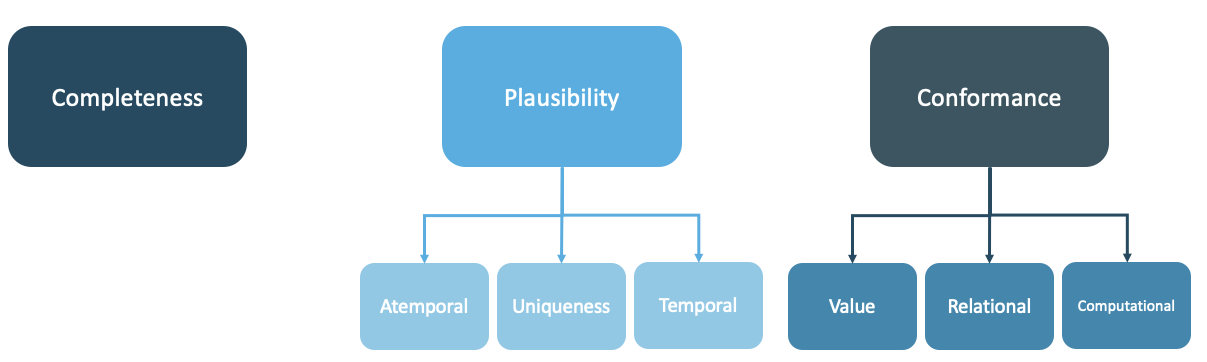
\includegraphics[scale=0.29]{figures/data-quality-v1.png}
\end{figure}
%TC:endignore
\subsection{Methods}
% !TeX root = ../../thesis.tex

For completeness, we used the inverse of the percentage of nulls in the training set. For plausibility, several methods were applied. The first was a Bayesian network. 

In our approach, Bayesian networks, which are probabilistic graphical models, play a pivotal role in predicting the plausibility of different elements. These networks are structured as directed acyclic graphs, where each node represents a variable and edges denote conditional dependencies among these variables \unskip~\cite{pearl1988probabilistic}. This structure allows the network to efficiently manage and represent the probabilistic relationships between multiple variables. The core strength of Bayesian networks in our context lies in their ability to predict the plausibility of various elements by analyzing these interdependencies. By integrating the conditional probabilities of variables and their dependencies, the network can infer the likelihood of certain outcomes or states, thereby assessing the plausibility of different columns in our dataset, when compared with the registered value. 

With this, we hope to capture the heterogeneous essence of the data, as well as possible outliers that are also plausible. We chose this model for its dual advantages: its capability to classify the plausibility of all columns within a single unified framework, and its interpretability, which allows for a clearer understanding of how each variable influences the overall plausibility prediction. The networks were created with the pgmpy package \unskip~\cite{pgmpy}. 

Secondly, we added the outlier-tree method\unskip~\cite{cortesExplainableOutlierDetection2020} which tries to integrate a decision tree that ''predicts'' the values of each column based on the values of each other column. In the process, every time separation is evaluated, it takes observations from each branch as a homogeneous cluster to search for outliers in the predicted 1-d distribution of the column. Outliers are determined according to confidence intervals in this 1-d distribution and need to have large gaps in order to be marked as outliers in the next observation. Because it looks for outliers in the branch of the decision tree, it knows the conditions that make it a rare observation relative to other observation types corresponding to the same conditions, and these conditions are always related to target variables (as predicted by them).  As such, it can only detect outliers described by decision tree logic, and unlike other methods such as isolation forests, it can not assign outlier points to each observation, or detect outliers that are generally rare, but will always provide human-readable justification when it recognizes outliers. Therefore, these methods not only identify anomalies based on a single column/variable but also consider the context of the data, providing a more nuanced understanding of what constitutes an outlier. This contextual awareness ensures that the outliers are not merely statistical deviations but are also substantively significant within the specific framework of the target variables. 

We added also elliptic envelope and Local Outlier Factor as complementary models to these two. Elliptic envelope is a method that assumes a Gaussian distribution of data, fitting an ellipse to the central data points to identify outliers. It works best with normally distributed data but is less effective in higher dimensions or non-normal distributions. Local Outlier Factor measures the local density deviation of a data point relative to its neighbors, identifying outliers without assuming a specific data distribution. It is versatile for different data structures but sensitive to parameter settings, like the number of neighbors. 

An Interquartile Range (IQR) based metric was also added as a supportive metric. This metric used the difference between Q1 and the triple of IQR  to define a lower threshold and Q3 + 3IQR to define an upper threshold. We only categorized as outlier the values that fell outside these margins. Finally, a rule system was implemented to leverage domain knowledge in the overall scoring. The system is based on great expectations package \unskip~\cite{GXProactiveCollaborative}. A set of 17 rules was defined by the team, focusing on impossible numbers or relationship between variables  or value format. The rules covered plausability and conformance. 

The Conformance-based were related to technical issues like the format of dates (date of birth like d/m/y), and conformance to the value set (i.e. Robson group, bishop scores, or delivery types). Plausibility rules were linked to expected values for BMI, weight, and gestational age (gestational age between 20 and 44). We also added plausibility for the relationship between columns, namely weight across different weeks of gestation (weight week 35 {\textgreater} weight week 25). We have also added a relationship of greatness between ultrasound weights more than 5 weeks apart. 

As for preprocessing, all null representations were standardized, we also removed features with high missing rates ({\textgreater} 80\% ). The imputation process was performed with the median for continuous and a new category (NULLIMP) for categorical variables.

For the usage of the Bayesian network in particular, the continuous variables were discretized into three bins defined by quantile. We defined three as the number of bins in order to reduce the number of states in each node of the network. The evaluation was done with cross-validation with 10 splits and two repetitions for each column as the target.

The API for serving the prediction models was developed with FastAPI. So, the methods applied in terms of the DQA framework shown in figure \ref{fig:categories} are described in the table \ref{tab:methods}.

\begin{table}[htpb]
\caption{Implemented Methods in the tool. The first column is the category or data quality dimension. The second is a subcategory of the first column if applicable and the third column is the actual method used to assess such a dimension.} \label{tab:methods}
\renewcommand{\arraystretch}{1.4}
\setlength{\tabcolsep}{10pt}

\begin{tabularx}{\textwidth}{ p{2cm} p{3.5cm} X }
\hline
 Category   & Subcategory           & Method   \\ \hline
Completeness     & N/A               & Score by the inverse percentage of missing in the train data         \\ 
Plausibility & Atemporal Plausibility & Bayesian model prediction based on the other values of row \\ 
Plausibility & Atemporal Plausibility         & Z-score for column value based on IQR train data       \\    
Plausibility & Atemporal Plausibility           & Elliptic Envelope                       \\ 
Plausibility & Atemporal Plausibility           & Local Outlier Factor                \\ 
Conformance & Value Conformance           & Manual Rule engine                           \\ 
Plausibility & Atemporal Plausibility           & Manual Rule engine                      \\ 
Plausibility & Atemporal Plausibility           & outlier-tree                      \\ 
Conformance & Value Conformance & Manual Rule engine\\
\hline
\end{tabularx}

\end{table}


For trying to compile all of these models into a single value, that could grasp the quality of the row or patient, a scoring method was created. The method of calculating the final score is stated in figure \ref{fig:scoring_method}. 
%TC:ignore
\begin{figure}[htbp]
    \centering
    \caption{Workflow and weights used for creating the final score and which elements are used to do so.}\label{fig:scoring_method} 
    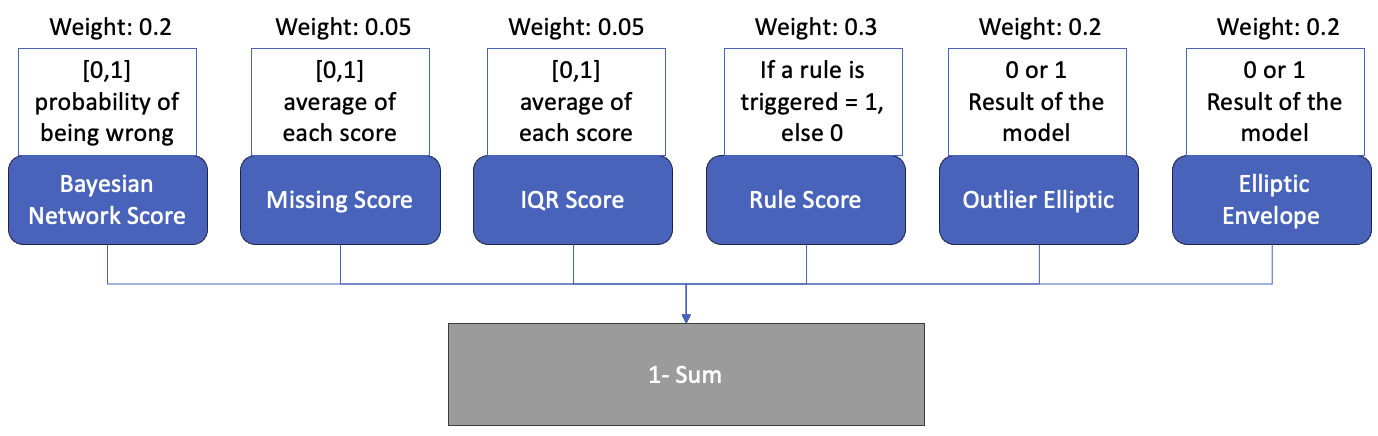
\includegraphics[scale=0.29]{figures/score-method.png}
    \end{figure}
    %TC:endignoregrama

To assess the tool's usefulness, we implemented it in a production environment and collect metrics regarding the data being produced. Then we presented some rows (or patient's records) to selected obstetrics clinicians for them to assess how likely the information is to be suitable for usage and rank it according to the perceived quality of the record. This was done through questionnaire, presenting the data and asking the clinicians to rank them from 1-10 and to describe the most important feature for the decision. We then compared the results with the ones from the model to make sanity checks regarding the model's performance and adequacy. We used Kendal Tau and Average Spearman's Rank Correlation Coefficient. Kendall Tau is a non-parametric statistic used to measure the strength and direction of the association between two ordinal variables. It calculates the difference between the number of concordant and discordant pairs of observations, normalized to ensure a value between -1 (perfect disagreement) and 1 (perfect agreement). Spearman's rank correlation coefficient is a non-parametric measure that assesses the strength and direction of a monotonic relationship between two ranked variables. It is based on the ranked values of the variables rather than their raw data, producing a value between -1 (perfect inverse relationship) and 1 (perfect direct relationship). Finally, we tested the capability of the model to discriminate bad quality records from good quality records, testing various thresholds of rank of quality, taken into account physicians responses.
We wrote all the code in Python 3.10.6 with the usage of the scikit-learn library for preprocessing, and evaluation\unskip~\cite{scikit-learn}.

\subsection{Results}

A \ac{bn} with structure and parameters learned from the training dataset reached an average \ac{auroc} of 0.857. The results are in the table \ref{tab:result_auc}.



\begin{table}[htpb]
 \caption{Validation Results: Column acronym with \ac{auroc} along with 95\% \ac{ci}. Acronym description is available in appendix \ref{appendix:data_dict}} \label{tab:result_auc} 

\renewcommand{\arraystretch}{1.2}
%\setlength{\tabcolsep}{8pt}
\centering
\begin{tabular} { p{1.5cm} p{1.5cm} p{3cm} p{1.5cm} p{1.5cm} l }
\hline
AP & 0.944 & [0.943, 0.945] & VNH & 0.894 & [0.893, 0.895] \\
AG & 0.797 & [0.778, 0.816] & TPEE & 0.816 & [0.815, 0.816] \\
EA & 0.969 & [0.968, 0.969] & AA & 0.751 & [0.743, 0.758] \\
CA & 0.958 & [0.958, 0.958] & GR & 0.931 & [0.93, 0.932] \\
IA & 0.638 & [0.637, 0.638] & V & 0.983 & [0.982, 0.983] \\
PI & 0.881 & [0.88, 0.881] & TP & 0.866 & [0.865, 0.868] \\
IMC & 0.881 & [0.881, 0.882] & VCS & 0.79 & [0.789, 0.791] \\
NRC & 0.75 & [0.75, 0.75] & ANP & 0.942 & [0.938, 0.946] \\
IGA & 0.968 & [0.968, 0.969] & GS & 0.514 & [0.507, 0.52] \\
SGP & 0.974 & [0.974, 0.974] & S & 0.896 & [0.896, 0.897] \\
VA & 0.974 & [0.974, 0.974] & VP & 0.771 & [0.77, 0.772] \\
TG & 0.728 & [0.726, 0.73] & TPNP & 0.952 & [0.951, 0.952] \\
\hline
 \multicolumn{6}{c}{\textbf{Average}  \textbf{0.857 [0.846, 0.868]}} \\

\hline
\end{tabular}
\end{table}


The network is as represented in figure \ref{fig:network}.
%TC:ignore
\begin{figure}[htbp]
\centering
\caption{Network learned}\label{fig:network} 
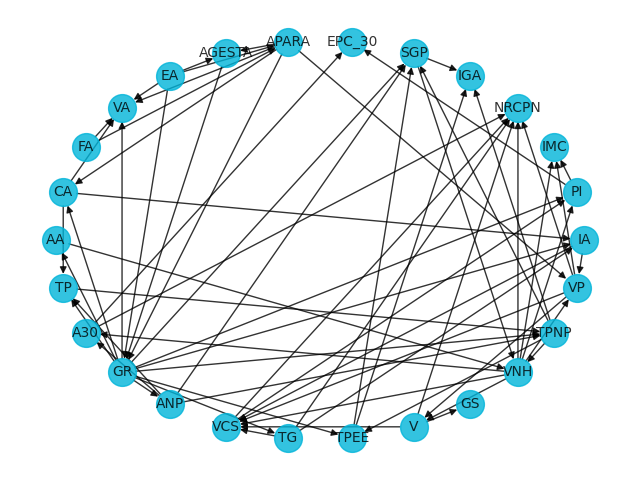
\includegraphics[scale=0.68]{figures/network.png}
\end{figure}
%TC:endignore

As for the rules created, they were conformance-based, like the format of dates, and conformance to the value set (i.e. Robson group, bishop scores, or delivery types). We also added plausibility rules, like expected values for BMI, weight, and gestational age. We also added plausibility for the relationship between columns, namely weight across different weeks of gestation. We have also added a relationship of greatness between ultrasound weights more than 5 weeks apart. 
The method of calculating the final score is stated in figure \ref{fig:wf}.


%TC:ignore
\begin{figure}[htbp]
    \centering
    \caption{Workflow for creating the final score and which elements are used to do so}\label{fig:wf} 
    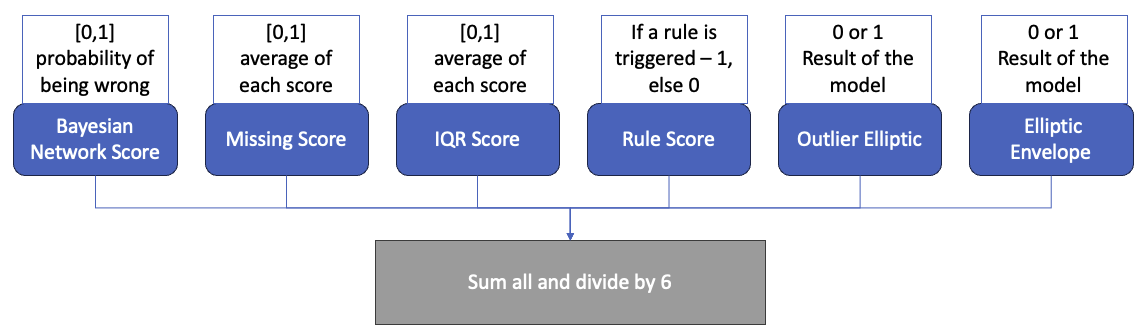
\includegraphics[scale=0.38]{figures/wf-update-dq.png}
    \end{figure}
    %TC:endignore


\subsection{Deployment \& Validation}
The purpose of this model is to serve as an \ac{api} for usage within a healthcare institution and act as a supplementary data quality assessment tool. Although a concrete, vendor-specific information model and health information system were initially used, our goal is to develop a more universal clinical decision support system. This system should be usable across all systems involved in birth and obstetrics departments. Therefore, we constructed it using the \ac{hl7} \ac{fhir} R5 version standard. This approach simplifies the process of API interaction. Rather than utilizing a proprietary model for the data, we based our decision on the use of \ac{fhir} resources: Bundle and Observation. These resources handle the request and response through a customized operation named "\$quality\_check". We intend to publish the profiles of these objects to streamline API access via standardized mechanisms and data models. The model then makes use of the customized operation and of several base resources to construct a \ac{fhir} message, which are: Bundle, MessageHeader, Observation, Device. Observation is where the information about the record is contained, Device contains information about the model, and MessageHeader is used to add information about the request. Finally, the Bundle is used to group all of these resources together. The current version of the profiles can be accessed here \cite{almeidaObstetricsClinicalDecision}.

For validation, we deployed the tool in docker format in a hospital to gather new data. We gathered 3231 new cases and returned a score for quality as exemplified in figure \ref{fig:scores}. Being that the score is from 0 to 1, the average score was 0.23 and \ac{iqr} was 0.03.
As for the clinicians' assessment, we got 4 answers. Figure \ref{fig:clinical} shows the aggregated rankings of the clinicians per record and is ordered by the rank provided by the model.



%TC:ignore
\begin{figure}[htbp]
\centering
\caption{Model score for newly seen data}\label{fig:scores} 
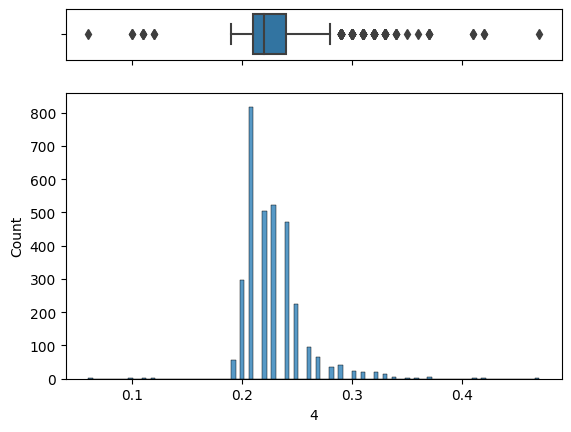
\includegraphics[scale=0.78]{figures/Scoring.png}
\end{figure}
%TC:endignore

%TC:ignore
\begin{figure}[htbp]
\centering
\caption{Comparison of clinical assessment of records with the model. Y is the clinicians' assessment, X is the ranking of the record per the model. Equal numbers on the X mean a tie per the model interpretation. Color is the record ID.}\label{fig:clinical} 
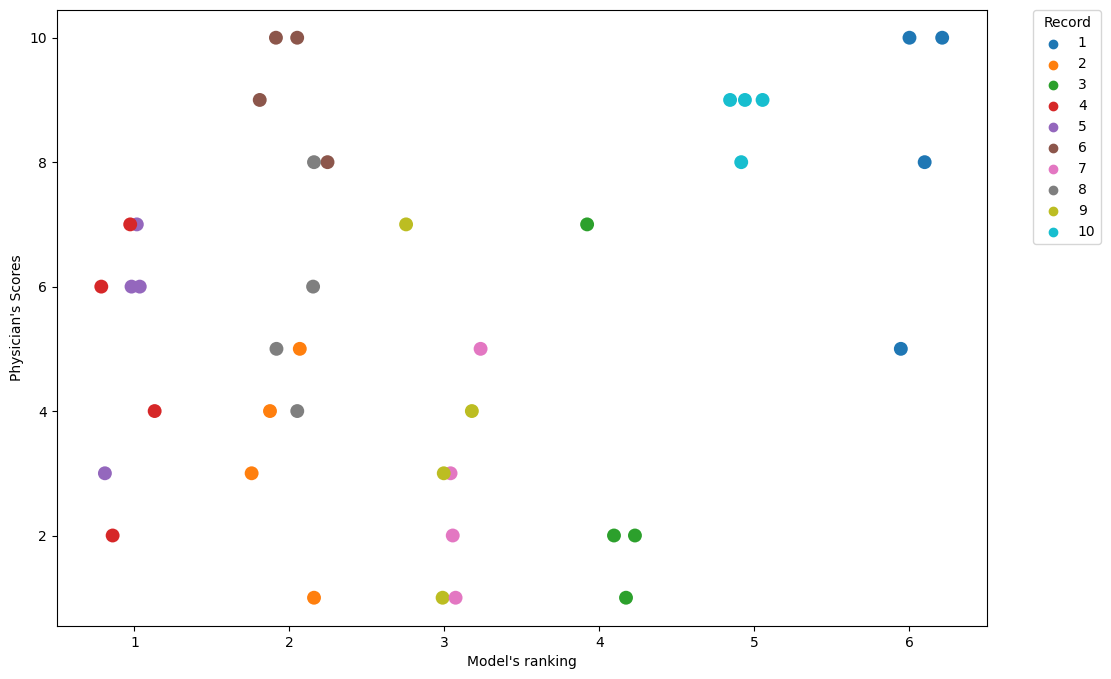
\includegraphics[scale=0.52]{figures/clinical_assessment_dataqual_scatter.png}
\end{figure}
%TC:endignore

The Average Spearman's Rank Correlation Coefficient was 0.04 and the Kendall's Tau was 0.0 with a \textit{\textit{P} value} of 1.

\subsection{Discussion}
% !TeX root = ../../thesis.tex
This work adds several pieces of information to the state of the art of data quality analysis. First we tried to map the output of an automatic assessment tool to the human perception of quality and the issues linked to doing so. Secondly, the fact that we applied \ac{xai} methods such as bayesian networks to leverage the potency of advanced data analysis without compromising interpretability and explainability. Furthermore, a single model was able to reach high performance metrics for almost all variables. Thirdly, the fact that interoperability standard such as \ac{fhir} can be adopted to facilitate the usage and information exchange of such tools. However, there are also shortcoming and challenges to address. The first is that data quality is still an elusive concept since it has a contextual dimension and the quality of the record depends on the usage of the information. For example, data aimed at primary usage and day-to-day healthcare decisions about a patient will have different requirements regarding the importance of some variable or completeness of information very different from data needed to create summary statistics for key performance indicators extraction. Moreover, the data is still very vendor-specific. Even though we used an interoperability standard, the semantic layer, more connected with terminology is still lacking. This is an issue to be addressed in order to improve the interoperability of the standard. Moreover, we do not know how the training done with this data is generalizable to other vendors. One opportunity arises of mapping all of this data to a widely used terminology like SNOMED CT or LOINC. Nevertheless, the usage of FHIR and the fact that the data is mapped to a standard terminology, makes it easier to use the data in other systems and to compare the results with other studies. Furthermore, being available freely and online makes it easier to understand how to map vendor-specific datasets to the model and use it in other contexts. Regarding the model, the usage of explainable methodologies like outlier-tree and transparent models like Bayesian networks are vital for clinical application. Since we use a single model to classify possible errors in the records, the ability to try to show clinicians why that value was tagged is of uttermost importance in order to get feedback and action from humans. From the experience gathered with the study, we believe that a weaker but transparent model could have more impact than better performant but opaque ones. If explainability and interpretability are important for any ML problem, this need only increases when we are dealing with such subjective concepts as data quality.

Regarding the clinical evaluation, we found that asking clinicians to purely assess the quality of a record in an \ac{ehr} is not an easy task. We discovered that for a proper assessment, a context and objective must be defined in order to make the evaluation more objective and manageable. Moreover, the ranking methodology, though very useful for comparison with the model, presents challenges for clinicians who find it difficult to order 10 records when some appear to be of equal quality. This is a very important aspect to consider when designing an evaluation method for data quality. Perhaps a categorical evaluation of yes/no would be more effective than ordering several records. These reasons might explain the great variability between clinicians (figure \ref{fig:clinical-dq}) and between clinicians and the model (Spearman and Kendall tau). Despite that, our preliminary results are promising, demonstrating an \ac{auroc} curve for categorizing bad quality records as high as 88\% and low as 56\%. The highest value was achieved by classifying all record with a mean rank of 4 or above as bad quality and the others as good quality records. However, these results rely on very few samples, so more data and research are needed in this area since it is a very subjective decision, and it should take into account the context and the objective of the evaluation. For example, if the objective is research use, the weights given to each dimension can be a set. On the other hand, if the objective is to use the data for day-to-day clinical decisions, another set of weights could be used. 

For the next steps, a promising research direction would be identifying contexts for applying data quality checks like primary usage, research purposes, and aggregated analysis for decision-making among others. This could enhance targeting those contexts and understanding the importance of each variable for those use cases. Incorporating this approach into the tool to weigh the different variables according to the context would be beneficial.  Finally, gaining access to more data and clinician evaluation of records, although challenging, is important to thoroughly assess the performance of the tool.


\subsection{Conclusion}
% !TeX root = ../../thesis.tex

We believe the work done is already a valuable insight into how to use data quality frameworks and several statistical tools in order to assess EHR data quality in real time. This is a fundamental process not only to guarantee the quality of data for primary usage but also for securing quality for secondary analysis and usage. We believe the fact that we created an interoperable tool that was trained on real obstetrics data from 9 different hospitals and has the ability to provide a single score for a clinical record can help institutions, academics, and EHR vendors implement data quality assessment tools in their own systems and institutions. With the further evaluation of the score and its relationship with clinical usefulness and a further assessment of a threshold for the score for defining a record that would require human attention would be vital to apply this tool in production with high levels of trust and quality.


